\PassOptionsToPackage{pdfpagelabels=false}{hyperref}
\documentclass[fleqn,usenatbib,usedcolumn]{mnras}
%==============================================================================%
\usepackage[british]{babel}             % British English hyphenation
\usepackage{txfonts}                  % Good fonts
% Use vector fonts, so it zooms properly in on-screen viewing software
% Don't change these lines unless you know what you are doing
%\usepackage[T1]{fontenc}
%\usepackage{ae,aecompl}
%%%%% AUTHORS - PLACE YOUR OWN PACKAGES HERE %%%%%
\usepackage{graphicx}	% Including figure files
\usepackage{hyperref} % hyperlinks
\usepackage{natbib}
\usepackage{aastexmacros}
\usepackage{tikz}
\usepackage[algoruled]{algorithm2e}
\usepackage[caption=false]{subfig}
\usepackage[mediumspace,mediumqspace,Grey,squaren]{SIunits}

%%%%%%%%%%%%%%%%%%%%%%%%%%%%%%%%%%%%%%%%%%%%%%%%%%

%%%%% AUTHORS - PLACE YOUR OWN COMMANDS HERE %%%%%
\usetikzlibrary{shapes,arrows,calc,positioning}

\renewcommand{\vec}[1]{\mathbf{#1}}
% \newcommand{\text}{\mathrm}
\newcommand{\jansky}{\text{Jy}}
\newcommand{\cheng}[1]{ {\color{teal}[{\bf Cheng TODO:~{#1}}]} }
\newcommand{\matthew}[2]{ {\color{white!20!violet}[{\bf TODO(#1):~{#2}}]} }
\newcommand{\todo}[1]{ {\color{red}[{\bf TODO:~{#1}}]} }
\newcommand{\edited}[1]{{\bf {#1}}}
\newcommand{\edit}[1]{{\bf Edit:~{#1}}}

\newcommand{\underset}[2]{\mathop{#2}\limits_{#1}}

\let\subsectionautorefname\sectionautorefname
\let\subsubsectionautorefname\sectionautorefname

\makeatletter
\newcommand\footnoteref[1]{\protected@xdef\@thefnmark{\ref{#1}}\@footnotemark}
\makeatother

\newcommand{\aref}[1]{\hyperref[#1]{Appendix~\ref{#1}}}

\AtBeginDocument{\def\chapterautorefname{Chapter}}%
\AtBeginDocument{\def\sectionautorefname{Section}}%
\AtBeginDocument{\def\subsectionautorefname{Section}}%
\AtBeginDocument{\def\algorithmautorefname{Algorithm}}%


%%%%%%%%%%%%%%%%%%%%%%%%%%%%%%%%%%%%%%%%%%%%%%%%%%

%%%%%%%%%%%%%%%%%%% TITLE PAGE %%%%%%%%%%%%%%%%%%%

\title[Machine learning for radio cross-identification]{Radio Galaxy Zoo: Machine learning for radio source host galaxy cross-identification}

\author[Alger et al.]{M.~J.~Alger$^{1, 2}$\thanks{Email: \href{mailto:matthew.alger@anu.edu.au}{matthew.alger@anu.edu.au}},
  J.~K.~Banfield$^{1, 3}$,
  C.~S.~Ong$^{2, 4}$,
  L.~Rudnick$^{5}$,
  O.~I.~Wong$^{6, 3}$,
  C.~Wolf$^{1, 3}$,
  \newauthor
  H.~Andernach$^{7}$,
  R.~P.~Norris$^{8, 9}$,
  S.~S.~Shabala$^{10}$
\\
% List of institutions
$^{1}$Research School of Astronomy and Astrophysics, The Australian National University, Canberra, ACT 2611, Australia\\
$^{2}$Data61, CSIRO, Canberra, ACT 2601, Australia\\
$^{3}$ARC Centre of Excellence for All-Sky Astrophysics (CAASTRO)\\
$^{4}$Research School of Computer Science, The Australian National University, Canberra, ACT 2601, Australia\\
$^{5}$Minnesota Institute for Astrophysics, University of Minnesota, 116 Church St. SE, Minneapolis, MN 55455\\
$^{6}$International Centre for Radio Astronomy Research-M468, The University of Western Australia, 35 Stirling Hwy, Crawley, WA 6009, Australia\\
$^{7}$Departamento de Astronom\'ia, DCNE, Universidad de Guanajuato, Apdo. Postal 144, CP 36000, Guanajuato, Gto., Mexico\\
$^{8}$Western Sydney University, Locked Bag 1797, Penrith South, NSW 1797, Australia\\
$^{9}$CSIRO Astronomy \& Space Science, PO Box 76, Epping, NSW 1710, Australia\\
$^{10}$School of Natural Sciences, University of Tasmania, Private Bag 37, Hobart, Tasmania 7001, Australia
}

% These dates will be filled out by the publisher
\date{Accepted XXX. Received XXX}

% Enter the current year, for the copyright statements etc.
\pubyear{2017}

% Don't change these lines
\begin{document}
\label{firstpage}
\pagerange{\pageref{firstpage}--\pageref{lastpage}}
\maketitle

% Abstract of the paper
\begin{abstract}
  Radio source host galaxy cross-identification is the problem of determining
  the host galaxies of radio sources. While this is possible by hand, manual
  cross-identification is intractable for wide-area radio surveys like the
  Evolutionary Map of the Universe (EMU). \edited{Automated
  cross-identification will be critical for these future surveys, and machine
  learning may provide the tools to develop such methods. We apply a standard
  approach from computer vision to cross-identification, introducing one
  possible way of automating this problem and exploring the pros and cons of
  this approach}. We apply our method to the $1.4$~GHz Australian Telescope
  Large Area Survey (ATLAS) observations of the \emph{Chandra} Deep Field
  South (CDFS) and the ESO Large Area ISO Survey South 1 (ELAIS-S1) fields,
  cross-identifying them with the \emph{Spitzer} Wide-area Infrared
  Extragalactic (SWIRE) survey. We train our method with two sets of training
  data: expert cross-identifications of CDFS from the initial ATLAS data
  release and crowdsourced cross-identifications of CDFS from Radio Galaxy
  Zoo. \edited{We found that while the estimated best-case performance from
  applying this method is near 100 per cent, a nearest-neighbour approach
  outperforms our trained methods. This is likely due to ATLAS containing a
  low number of extended radio sources and so our method does not see enough
  complex examples to learn to accurately cross-identify them. Much larger
  datasets are therefore required for training methods like ours. We also show
  that training our method on Radio Galaxy Zoo cross-identifications gives
  comparable results to training our method on expert cross-identifications,
  demonstrating the value of crowdsourced training data.}
\end{abstract}

% Select between one and six entries from the list of approved keywords.
% Don't make up new ones.
\begin{keywords}
methods: statistical -- techniques: miscellaneous -- galaxies: active -- radio continuum: galaxies -- infrared: galaxies\\
\end{keywords}

%%%%%%%%%%%%%%%%%%%%%%%%%%%%%%%%%%%%%%%%%%%%%%%%%%
%%%%%%%%%%%%%%%%% BODY OF PAPER %%%%%%%%%%%%%%%%%%

\section{Introduction}\label{introduction}

  \begin{figure}
  \begin{center}
    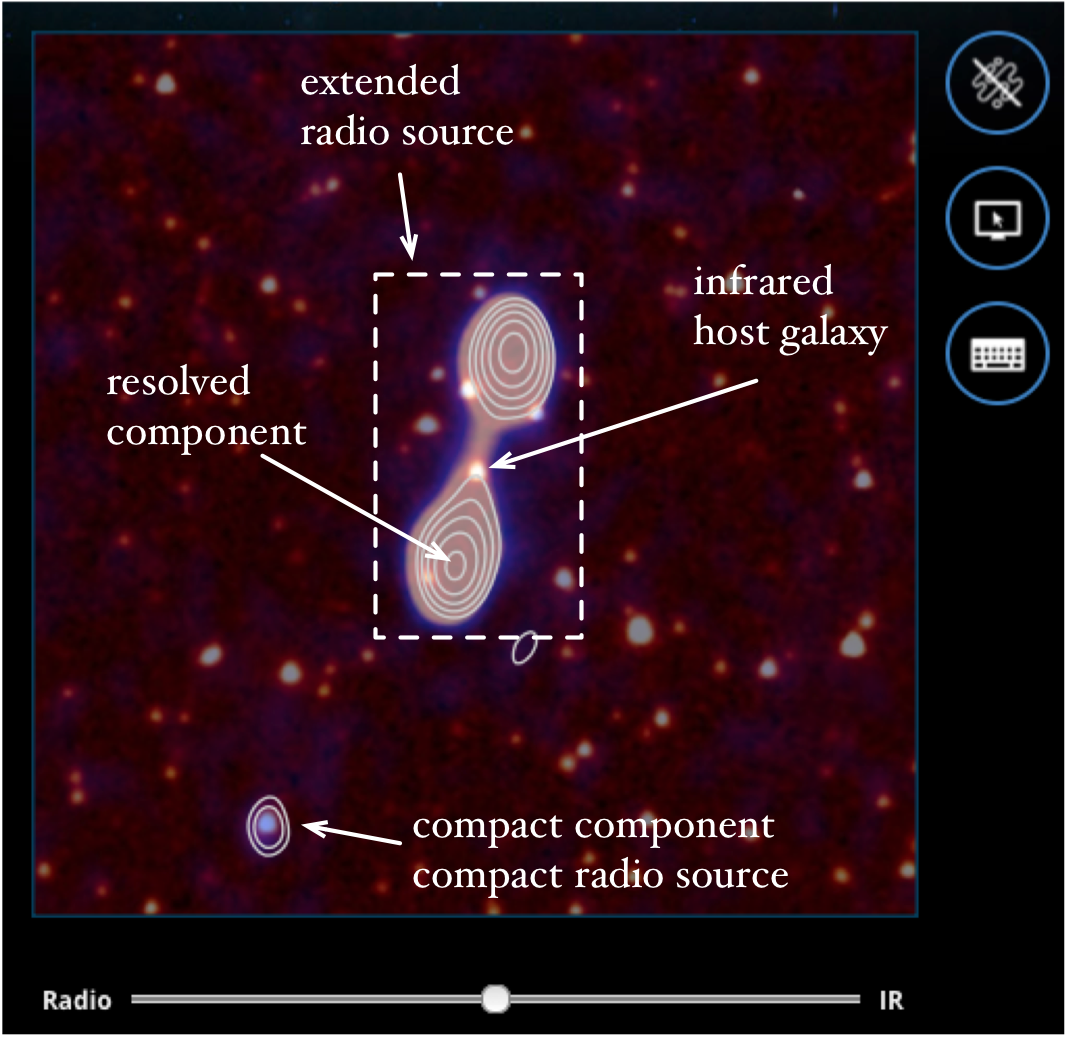
\includegraphics[width=0.75\linewidth]{images/fig1.png}
    \caption{Key definitions of radio emission regions used throughout this paper.}\label{fig:definitions}
  \end{center}
  \end{figure}

  Next generation radio telescopes such as the Australian SKA Pathfinder
  \citep[ASKAP;][]{johnston07} and Apertif \citep{verheijen08} will conduct
  increasingly wide, deep, and high-resolution radio surveys, producing large
  amounts of data. The Evolutionary Map of the Universe
  \citep[EMU;][]{norris11} survey using ASKAP is expected to detect over 70 million
  radio sources, compared to the 2.5 million radio sources currently
  known \citep{banfield15}. An important part of processing these data is cross-identifying observed
  radio emission regions with observations of their host galaxy in surveys at
  other wavelengths.

  Cross-identification of the host with extended radio emission can be a
  difficult task. \edited{Radio emission may extend far from the host galaxy
  and emission regions from a single physical object may appear disconnected
  due to interferometry `resolving out' diffuse structure. As a result, the
  observed structure of a radio source may have a complex relationship
  with the corresponding host galaxy, and cross-identification in radio is
  much more difficult than cross-identification at shorter wavelengths.} Small surveys
  containing a few thousand sources such as the Australia Telescope Large Area Survey
  \citep[ATLAS;][]{norris06, middelberg08} can be cross-identified manually,
  but this is impractical for larger surveys. New approaches must be found.

  One approach to cross-identification is crowdsourcing, where volunteers
  cross-identify radio sources with their host galaxy. This is the premise of Radio Galaxy
  Zoo\footnote{\url{https://radio.galaxyzoo.org}} \citep{banfield15}, a
  citizen science project hosted on the Zooniverse platform \citep{lintott08}.
  Volunteers are shown radio and infrared images and are asked to
  cross-identify radio sources with the corresponding infrared host galaxies. An
  explanation of the project can be found in \citet{banfield15}. The first
  data release for Radio Galaxy Zoo will provide a large dataset of over
  75~000 radio-host cross-identifications and radio source morphologies
  (Wong et al., in prep). While this is a much larger number of visual
  cross-identifications than have been made by experts \citep[e.g.,
  ][]{Taylor2007,Gendre2008,Grant2010,norris06,middelberg08} it is still far
  short of the millions of radio sources expected to be detected in upcoming
  radio surveys \citep{norris17surveys}.

  Automated algorithms have been developed for cross-identification.
  \citet{fan15} developed a method of cross-identification using Bayesian
  hypothesis testing, fitting a three-component model to extended radio
  sources. This was achieved under the assumption that extended radio sources
  are composed of a core radio component and two lobe components. The core
  radio component is coincident with the host galaxy, so cross-identification
  amounts to finding the galaxy coincident with the core radio component in
  the most likely model fit. This method is easily extended to use other, more
  complex models, but it is purely geometric. It does not incorporate
  other information such as the physical properties of the potential host
  galaxy. Additionally, there may be new classes of radio source detected in
  future surveys like EMU which do not fit the model. \citet{weston18lrpy}
  developed a modification of the likelihood ratio method of
  cross-identification \citep{richter75likelihood} for application to ATLAS
  and EMU. This method does well on non-extended radio sources
  with approximately 70 per cent accuracy in the ATLAS fields, but does
  not currently handle more complex (extended or multi-component) radio sources
  \citep{norris17unexpected}.

  \edited{One possibility is that machine learning techniques can
  be developed to automatically cross-identify surveys}. Machine learning
  describes a class of methods that learn approximations to functions. \edited{If
  cross-identification can be cast as a function approximation problem, then machine learning will allow data
  sets such as Radio Galaxy Zoo to be generalised to work on new data.}

  In this paper we \edited{cast cross-identification as a function
  approximation problem by} applying an approach from computer vision
  literature. This approach casts cross-identification as the standard machine
  learning problem of binary classification \edited{by asking whether a given
  infrared source is the host galaxy or not}. We train our methods on expert
  cross-identifications and volunteer cross-identifications from Radio Galaxy Zoo. In
  \autoref{sec:data} we describe the data we use to train our methods. In
  \autoref{sec:method} we discuss how we cast the radio host galaxy
  cross-identification problem as a machine learning problem. In
  \autoref{sec:results} we present results of applying our method to ATLAS
  observations of the \emph{Chandra} Deep Field South (CDFS) and in
  \autoref{sec:elais} we apply the cross-identifiers trained on CDFS to the
  ESO Large Area ISO Survey South 1 (ELAIS-S1) field. Our data and code are
  available at \url{https://radiogalaxyzoo.github.io/atlas-xid}.

  \edited{Throughout this paper, a `radio source' refers to all radio emission observed from
  a physical entity, and a `radio component' refers to a single connected
  observation of radio emission. Multiple components may comprise a single
  source. A `compact' source is composed of a single compact component and we
  assume that all unresolved components are compact sources. An `extended'
  source is a non-compact source, i.e. resolved single-component sources and
  multi-component sources. \autoref{fig:definitions} illustrates these definitions.}

\section{Data}\label{sec:data}

  We use radio data from the Australia Telescope Large Area Survey
  \citep[ATLAS;][]{norris06,franzen15}, infrared data from the \emph{Spitzer}
  Wide-area Infrared Extragalactic survey \citep[SWIRE;][]{lonsdale03swire,
  surace05swire}, and cross-identifications of these surveys from the citizen
  science project Radio Galaxy Zoo \citep{banfield15}. Radio Galaxy Zoo also
  includes cross-identifications of Faint Images of the Radio Sky at
  Twenty-Centimeters \citep[FIRST;][]{white97first} and the All\emph{WISE}
  survey \citep{cutri2013wiseexplanatory}, though we focus only on Radio
  Galaxy Zoo data from ATLAS and SWIRE.

  \subsection{ATLAS}\label{sec:atlas}
    \begin{table}
      \caption{Catalogues of ATLAS/SWIRE cross-identifications for the CDFS
        and ELAIS-S1 fields. The method used to generate each catalogue is
        shown, along with the number of radio components cross-identified in each
        field.}
      \label{tab:atlas-cids}
      \begin{tabular}{llcc}
        \hline
        Catalogue & Method & CDFS & ELAIS-S1\\
        \hline
        \citet{norris06} & Manual & 784 & 0\\
        \citet{middelberg08} & Manual & 0 & 1366\\
        \citet{fan15} & Bayesian models & 784 & 0\\
        \citet{weston18lrpy} & Likelihood ratio & 3078 & 2113\\
        Wong et al. (in prep) & Crowdsourcing & 2460 & 0 \\
        \hline
      \end{tabular}
    \end{table}

    ATLAS is a pilot survey for the EMU \citep{norris11} survey, which will
    cover the entire sky south of $+30$ deg and is expected to detect
    approximately 70 million new radio sources. \edited{95 per cent of these sources
    will be single-component sources, but the remaining 5 per cent provide
    considerable challenge to current automated cross-identification methods
    \citep{norris11}.} EMU will be conducted at the same depth and resolution
    as ATLAS, so methods developed for processing ATLAS data are expected to
    work for EMU. ATLAS is a wide-area radio survey of the CDFS and ELAIS-S1
    fields at 1.4~GHz with a sensitivity of 14 and
    \unit{17}{\micro\jansky}~beam$^{-1}$ on CDFS and ELAIS-S1 respectively.
    CDFS covers 3.6~deg$^2$ and contains 3034 radio components above a
    signal-to-noise ratio of 5. ELAIS-S1 covers 2.7~deg$^2$ and contains 2084
    radio components above a signal-to-noise ratio of 5 \citep{franzen15}. The
    images of CDFS and ELAIS-S1 have angular resolutions of 16 by 7 and 12 by
    8 arcsec respectively, with pixel sizes of 1.5 arcsec px$^{-1}$.
    \autoref{tab:atlas-cids} summarises catalogues that contain
    cross-identifications of radio components in ATLAS with host galaxies in
    SWIRE. In the present work, we train methods on
    CDFS\footnote{\edited{Radio Galaxy Zoo only contains CDFS sources and so
    we cannot train methods on ELAIS-S1.}} and test these methods on both CDFS
    and ELAIS-S1. This ensures our methods are transferable to different
    areas of the sky observed by the same telescope as will be the case for
    EMU.

  \subsection{SWIRE}\label{sec:swire}

    SWIRE \citep{lonsdale03swire, surace05swire} is a wide-area infrared
    survey at the four IRAC wavelengths 3.6, 4.5, 5.8, and
    \unit{8.0}{\micro\meter} \citep{lonsdale03swire}. It covers eight fields, including CDFS and ELAIS-S1. SWIRE is the source of infrared
    observations for cross-identification with ATLAS. SWIRE catalogues 221~535
    infrared objects in CDFS and 186~059 infrared objects in ELAIS-S1 above a signal-to-noise ratio of 5.

  \subsection{Radio Galaxy Zoo}\label{sec:rgz}

    Radio Galaxy Zoo asks volunteers to cross-identify radio components with
    their infrared host galaxies. There are a total of 2460 radio components
    in Radio Galaxy Zoo sourced from ATLAS \edited{observations of CDFS}. These components are
    cross-identified by Radio Galaxy Zoo participants with host galaxies
    detected in SWIRE. A more detailed description can be found in
    \citet{banfield15} and a full description of how the Radio Galaxy Zoo catalogue used in this work\footnote{The Radio Galaxy Zoo Data
    Release 1 catalogue will only include cross-identifications for which over
    65 per cent of volunteers agree. However, we use a preliminary catalogue containing volunteer
    cross-identifications for all components.} is generated can be found in Wong
    et al. (in prep).

    The ATLAS~CDFS radio components that appear in Radio Galaxy Zoo \edited{are drawn from a prerelease version of} the third data release
    of ATLAS by \citet{franzen15}. In this release, each radio component was fit with a
    two-dimensional Gaussian. Depending on the residual of the fit, more than
    one Gaussian may be fit to one region of radio emission. Each of these
    Gaussian fits is listed as a radio component in the ATLAS component catalogue. The
    brightest radio component from the multiple Gaussian fit is called the
    `primary component'. Each primary component found in the ATLAS
    component catalogue appears in Radio Galaxy Zoo. Non-primary components
    may appear within the image of a primary component, but do not have their
    own entry in Radio Galaxy Zoo. We will henceforth only discuss the primary
    components.

  \section{Method}\label{sec:method}
    \begin{figure}
      \centering
      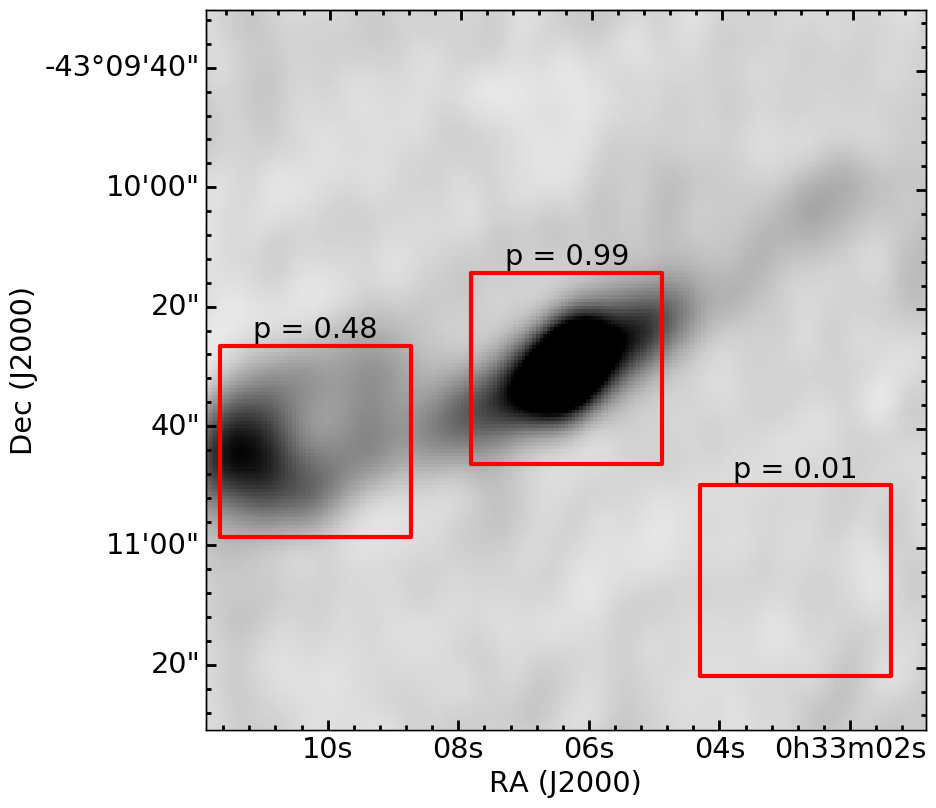
\includegraphics[width=\columnwidth]{images/fig2-jkb.png}
      \caption{An example of localising the host galaxy of a radio source using
        our method. This image is a radio image from ATLAS and is centred on
        $\alpha = 00^\text{h}33^\text{m}06.36^\text{s}, \delta =
        -43^\circ{}10'30.1''$. Boxes represent $32 \times 32$ pixel `windows'
        centred on various locations in the image. \edited{Each window} is used to represent the location that the window is centred
        on. The probabilities of each window coinciding with the host galaxy
        would then be estimated by a \edited{binary classifier which maps windows to probabilities}. The probabilities
        shown are for illustration only. In this example, \edited{the galaxy coincident with the centre window would be chosen as the host galaxy, as this
        window has the highest probability}. \todo{Overlay radio over a greyscale IR image.}}
      \label{fig:windows}
    \end{figure}

  \subsection{Cross-identification as binary classification}\label{cross-identification-as-binary-classification}
    \begin{figure}
      \centering
      % http://www.texample.net/tikz/examples/simple-flow-chart/
      \tikzstyle{decision} = [diamond, draw, fill=white,
          text width=4.5em, text badly centered, inner sep=0pt]
      \tikzstyle{block} = [rectangle, draw, fill=white,
          text width=5em, text centered, rounded corners, minimum height=4em]
      \tikzstyle{line} = [draw, -latex']
      \begin{tikzpicture}[node distance=6mm, auto]
        \node [block] (init) {input radio source};
        \node [decision, right= of init] (iscompact) {compact?};
        \node [block, below= of iscompact] (compact) {find nearest infrared object};
        \node [block, right= of iscompact] (resolved) {find nearby infrared objects};
        \node [block, fill=black!30, right= of resolved] (classify) {classify objects};
        \node [block, below= of classify] (best) {choose object based on probability};
        \coordinate (middle) at ($(compact)!0.5!(best)$);
        \node [block, below= of middle, fill=green!40] (done) {\textbf{host galaxy}};
        \path [line] (init) -- (iscompact);
        \path [line] (iscompact) -- (compact) node [midway] {yes};
        \path [line] (compact) -- (done);
        \path [line] (iscompact) -- (resolved) node [midway] {no};
        \path [line] (resolved) -- (classify);
        \path [line] (classify) -- (best);
        \path [line] (best) -- (done);
      \end{tikzpicture}
      \caption{A cross-identification method employing a binary classifier. As
        input we accept a radio source. If the source is compact, we select
        the nearest infrared object as the host galaxy. If the source is
        resolved, we classify all infrared objects nearby within radius $R$
        and select the highest probability object as the host galaxy. The grey
        box is the classifier, which can be any binary classifier that outputs
        a probability.}
      \label{fig:flowchart}
    \end{figure}

    \begin{algorithm}
        \KwData{\\\quad{}A $2 \times 2$ arcmin radio image of a radio component%
                \\\quad{}A set of infrared candidate host galaxies $\mathcal G$%
                \\\quad{}A binary classifier $f : \mathbb R^d \to [0, 1]$}
        \KwResult{A galaxy $g \in \mathcal G$}

        $max \leftarrow -\infty$\;
        $host \leftarrow \emptyset$\;
        \For{$g \in \mathcal G$}{
          $x \leftarrow$ a $d$-dimensional vector representation of $g$ (\autoref{vector-representation-of-infrared-sources})\;
          $d \leftarrow$ distance between $g$ and the radio component\;
          $score \leftarrow f(x) \times \frac{1}{\sqrt{2\pi\sigma^2}} \exp\left(-\frac{d^2}{2\sigma^2}\right)$\;
          \If{$score > max$}{
            $max \leftarrow score$\;
            $host \leftarrow g$\;
          }
        }

        \KwRet{$host$}
        \caption{Cross-identifying a radio component given an image of the component, a catalogue of infrared candidate host galaxies and a binary classifier.}
        \label{alg:xid}
    \end{algorithm}

    We propose a two-step method for host galaxy cross-identification
    \edited{which we will derive now. Given a radio component, we want to find
    the corresponding host galaxy as a human would. The input is a $2' \times
    2'$ radio\footnote{Other wavelengths --- notably infrared --- might be
    useful, but we defer this for now as it complicates the task. Infrared
    information is instead incorporated separately in our method.} image of
    the sky centred on a radio component, matching the size of the images used
    by Radio Galaxy Zoo. To avoid solving the separate task of identifying
    which radio components are associated with the same source, we make the
    assumption that each radio image represents a single, complex extended
    source\footnote{Limitations of this assumption are discussed in
    \autoref{sec:limitations}.}. The radio cross-identification task can then
    be formalised as follows: given a radio image centred on a radio
    component, locate the host galaxy of the source containing this radio
    component. This is a standard computer vision problem called \emph{object
    detection}, and we apply a common technique called a \emph{sliding window}
    \citep{rowley1996facedetection}}.

    \edited{In sliding window object detection, the
    goal is to estimate the probability that each pixel in an image coincides
    with the desired object. Square cutouts (called \emph{windows}) are taken
    centred on each pixel and these cutouts are used to represent that pixel.
    We then estimate the probability that a given cutout is centred on the
    object that we want to find. To find the object, we then choose the pixel
    with maximum probability. To improve the efficiency of this process, we
    only consider cutouts centred on infrared sources --- otherwise we have to
    estimate probabilities for every pixel in the image\footnote{This approach
    implicitly assumes that host galaxies are always visible in the infrared,
    an assumption we discuss in \autoref{sec:limitations}.}. We call these
    infrared sources \emph{candidate host galaxies}. Using candidate host
    galaxies instead of pixels also allows us to include ancillary information
    about the candidate host galaxies, such as their infrared colours and
    redshifts.}

    \edited{A common method in machine learning is \emph{binary
    classification}, where objects are to be assigned to one of two classes,
    called the \emph{positive} and \emph{negative} classes. This assignment is
    represented by the probability that an object is in the positive class. A
    \emph{binary classifier} is a function mapping from an object to such a
    probability. Our formulation of cross-identification is equivalent to
    binary classification of candidate host galaxies: the positive class
    represents host galaxies, the negative class represents non-host galaxies,
    and to cross-identify a radio component we find the candidate host galaxy
    maximising the positive class probability. We therefore split
    cross-identification into two separate tasks: the \emph{galaxy
    classification task} where, given a candidate host galaxy, we wish to
    determine whether it is a host galaxy of \emph{any} radio component; and
    the \emph{cross-identification task} where, given a specific radio
    component, we wish to find its host galaxy. The galaxy classification task
    is a traditional machine learning problem which results in a binary
    classifier. The cross-identification task maximises over probabilities
    output by this classifier. Our approach is illustrated in
    \autoref{fig:windows} and described in \autoref{alg:xid}. We refer to the
    binary classifier mapping from a candidate host galaxy to a probability as
    $f$. To implement $f$ as a function that accepts candidate host galaxies
    as input, we need to represent candidate host galaxies by vectors. We
    describe this in \autoref{vector-representation-of-infrared-sources}.
    There are many options for modelling $f$. In this paper we apply three
    different models: logistic regression, random forests and convolutional
    neural networks.}

    \edited{We cross-identify each radio component in turn. The classifier $f$
    provides a score for each candidate host galaxy. This score indicates how
    much the candidate looks like a host galaxy, irrespective of which radio
    component we are cross-identifying. If there are other nearby host
    galaxies, then multiple candidate hosts may have high scores (e.g.
    \autoref{fig:broken-isolation}). The classifier is totally independent of
    which radio component we are cross-identifying. This is necessary to be
    able to find a binary classifier in the galaxy classification task --- we
    need multiple positive examples (i.e. host galaxies) to train a model, but
    for any specific radio component there is only one host galaxy. As a
    result, the galaxy classification task aims to answer the general question
    of whether a given galaxy is the host galaxy of \emph{any} radio
    component, while the cross-identification task attempts to cross-identify
    a \emph{specific} radio component. To distinguish between candidate host
    galaxies with high scores, we weight the scores by a Gaussian function of
    angular separation between the candidates and the radio component.} The
    width of the Gaussian, $\sigma$, controls the influence of the Gaussian on
    the final cross-identification. When $\sigma$ is small, our approach is
    equivalent to a nearest-neighbours approach where we select the nearest
    infrared object to the radio component as the host galaxy. In the limit
    where $\sigma \to \infty$, we maximise the probability output by the
    classifier as above. We take $\sigma = 30''$ as this was the best value
    found by a grid search.

    \edited{We can improve upon this method by cross-identifying compact radio sources
    separately to extended sources, as compact sources are much easier to
    cross-identify. For a compact source, the nearest SWIRE object may be
    identified as the host galaxy (a \emph{nearest-neighbours} approach), or a
    more complex method such as likelihood ratios may be applied
    \citep[see][]{weston18lrpy}. We cross-identify compact sources separately
    in our pipeline and this process is shown in \autoref{fig:flowchart}.}

  \subsection{Limitations of our approach}
    \label{sec:limitations}

     \begin{figure}
      \centering
      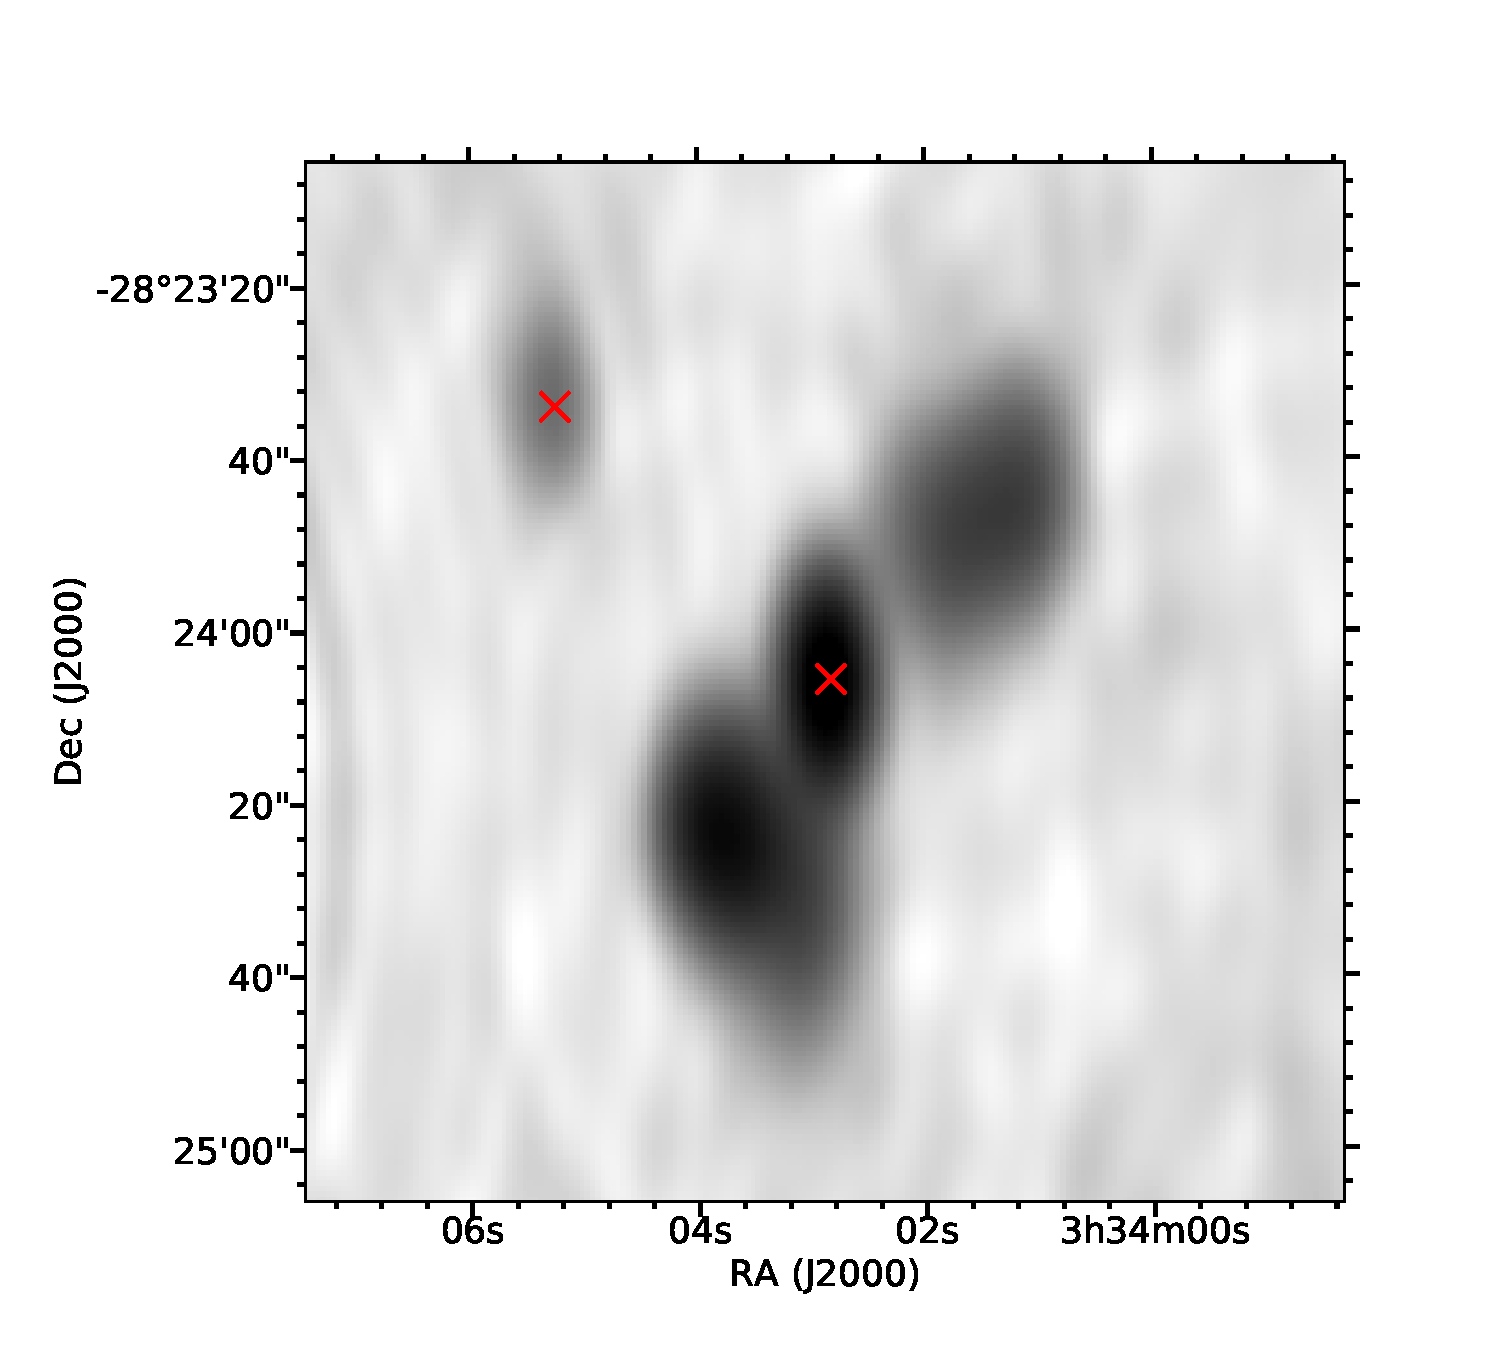
\includegraphics[width=\linewidth]{images/CI0077C1_fig.pdf}
      \caption{$2'$-wide radio image centred on ATLAS3\textunderscore{}J033402.87-282405.8C.
        %(ARG0003r2v)
        This radio source breaks the assumption that there are no other radio
        sources within 1~arcmin of the source. Another radio source is visible
        to the upper-left. Host galaxies found by Radio Galaxy Zoo volunteers
        are shown by crosses.}
      \label{fig:broken-isolation}
    \end{figure}

      \begin{figure}
      \centering
      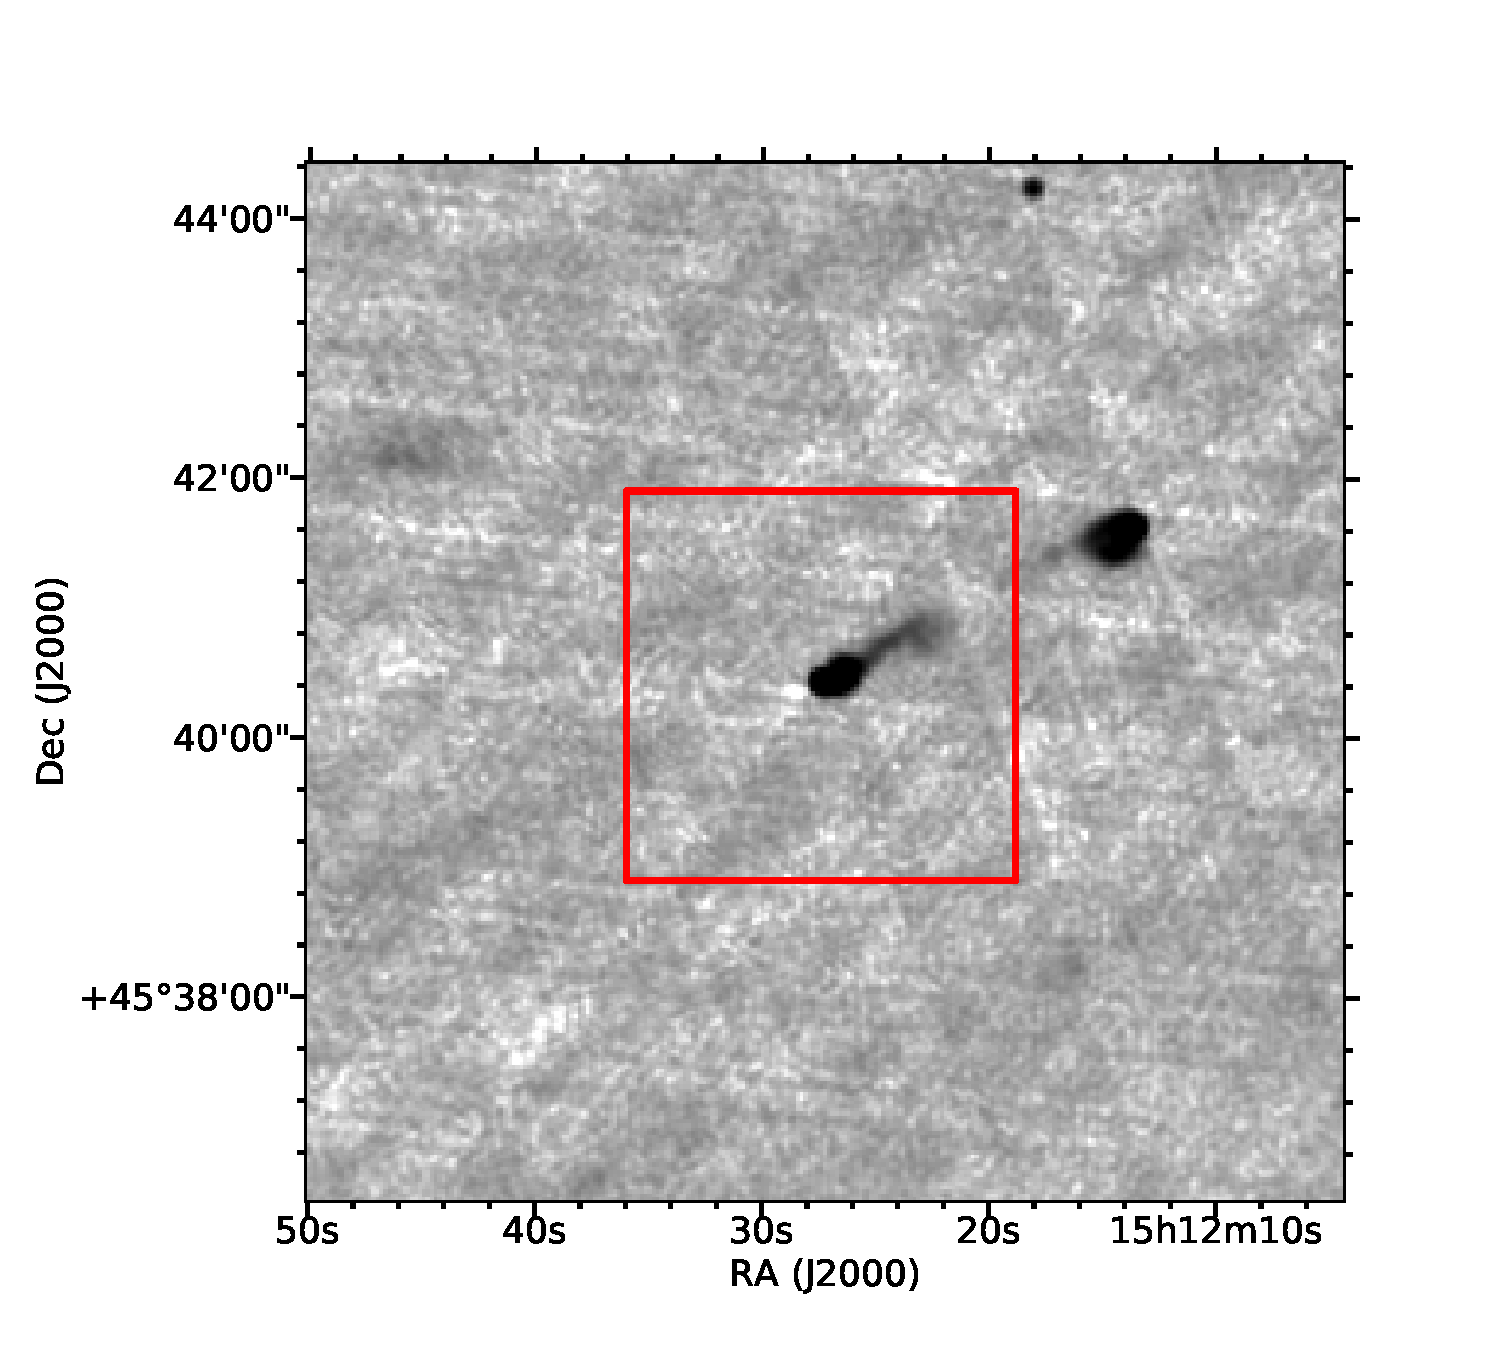
\includegraphics[width=\linewidth]{images/FIRSTJ151227_fig.pdf}
      \caption{A $8'$-wide radio image from FIRST, centred on
        FIRSTJ151227.2+454026. The $3'$-wide red box indicates the boundaries of
        the image of this radio component shown to volunteers in Radio Galaxy
        Zoo. This radio source breaks our assumption that the whole radio source
        is visible in the chosen radius. As one of the lobes of the radio source
        is outside of the image, a volunteer (or automated algorithm) looking at
        the $3'$-wide image may be unable to determine that this is a radio
        double or locate the host galaxy.}
      \label{fig:broken-contains}
    \end{figure}
        \begin{figure}
      \centering
      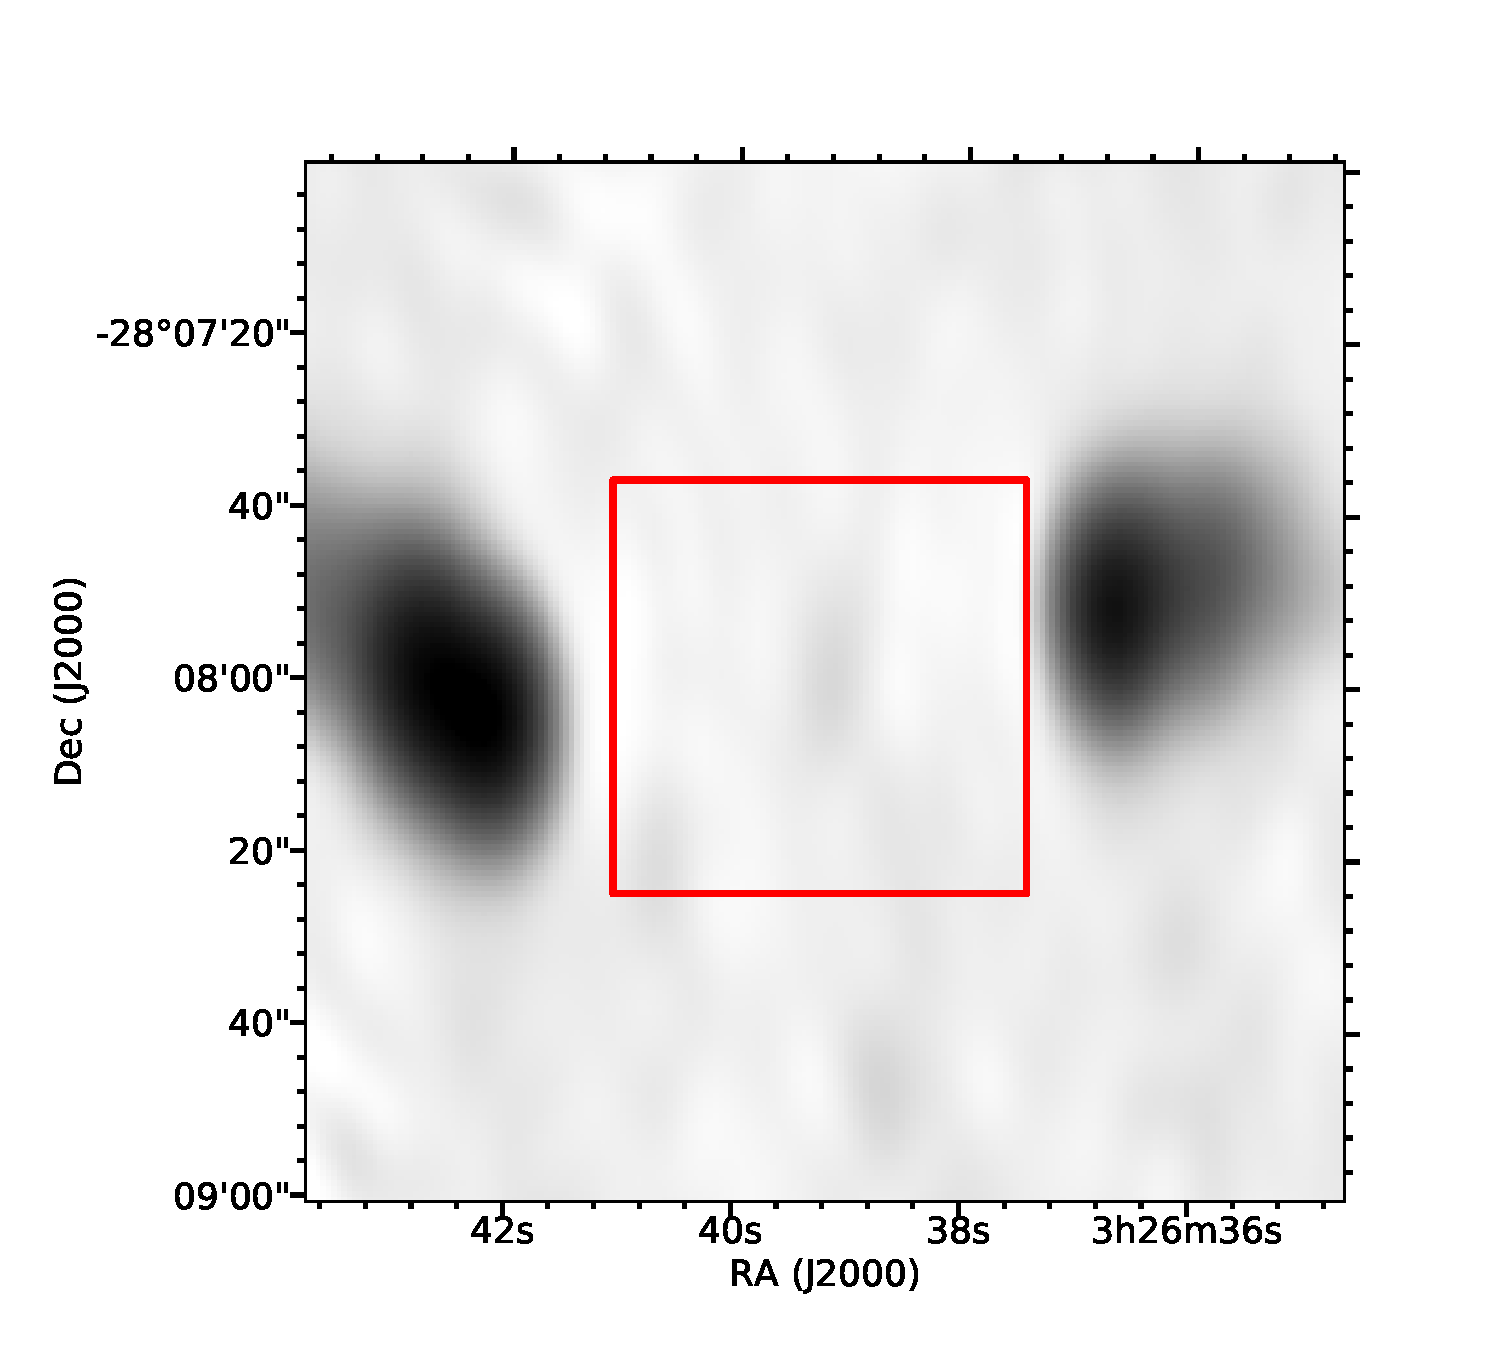
\includegraphics[width=\linewidth]{images/CI2363_fig.pdf}
      \caption{A radio image centred on $\alpha =
        03^\text{h}26^\text{m}39.12^\text{s}$, $\delta = -28^\circ{}07'58.80''$.        %ARG0003sky
        This is an example of a radio source where the window centred on the
        host galaxy, shown as a rectangle, does not contain enough radio
        information to correctly identify the galaxy as the host.}
      \label{fig:broken-window-size}
    \end{figure}

    We make a number of assumptions to relate the cross-identification task to
    the galaxy classification task:
    \begin{itemize}
      \item A radio image represents a whole, single radio source.
      \item The host galaxy of a radio component is within 1~arcmin of the
        component.
      \item The host galaxy of a radio component is closer on the sky to the
        radio component than the host galaxy of any other radio component.
      \item The host galaxy appears in the SWIRE catalogue.
    \end{itemize}
    These assumptions limit the effectiveness of our approach, regardless of
    how accurate our binary classification may be.

    \edited{The main limitations are problems of scale in choosing the
    candidate search radius and the size of the radio image cutouts
    representing candidates. If the search radius is too small, we may not
    consider the host galaxy as a candidate. If the search radius is too
    large, we may consider multiple host galaxies (though this is somewhat
    mediated by the Gaussian multiplier). If the cutout is too small, radio
    emission may extend past the edges of the window and we may miss critical
    information required to identify the galaxy as a host galaxy. If the
    cutout is too large, then irrelevant information will be included and it
    may be difficult or computationally expensive to classify. We chose a
    window size of $32 \times 32$ pixels, corresponding to approximately $48'' \times 48''$ in
    ATLAS. This is shown as red rectangles in \autoref{fig:windows} and
    \autoref{fig:broken-window-size}. These kinds of size problems are
    difficult even for non-automated methods as radio sources can be extremely
    wide --- for example, Radio Galaxy Zoo found a radio giant that spanned
    over three different images presented to volunteers and the full source
    was only cross-identified by the efforts of citizen scientists
    \citep{banfield15}. An example of a radio image where part of the radio
    source is outside the search radius is shown in
    \autoref{fig:broken-contains}.}

    In weighting the classification scores by a Gaussian function of angular
    separation, we implicitly assume that the host galaxy of a radio component
    is closer to that radio component than any other host galaxy. If this
    assumption fails then the incorrect host galaxy may be identified, though
    this is fairly rare.

    We only need the assumption that the host galaxy appears in SWIRE to
    incorporate galaxy-specific features
    (\autoref{vector-representation-of-infrared-sources}) and to improve
    efficiency. Our method is applicable even to radio sources not detected in
    the infrared by considering every pixel of the radio image as a candidate
    location as would be done in the original computer vision approach.

    Our assumptions impose an upper bound on how well we can cross-identify
    radio sources. We estimate this upper bound in \autoref{sec:cdfs-results}.

  \subsection{Feature vector representation of infrared sources}
  \label{vector-representation-of-infrared-sources}

    \edited{Inputs to binary classifiers must be represented by an array of real values called feature vectors.} We therefore need to choose a feature vector representation of our candidate host galaxies. Candidate hosts are sourced from the SWIRE catalogue (\autoref{sec:swire}). We represent each candidate host with 1034 real-valued features, \edited{combining the cutouts described in \autoref{cross-identification-as-binary-classification} and infrared ancillary data from the SWIRE catalogue}. For a given candidate host, these features are:
    \begin{itemize}
      \item the 6 logarithms of the ratios of fluxes of the candidate
        host at the four IRAC wavelengths;
      \item the flux of the host at \unit{3.6}{\micro\meter};
      \item the stellarity index of the host at both 3.6 and
        \unit{4.5}{\micro\meter};
      \item the radial distance between the candidate host and the nearest
        radio component in the ATLAS catalogue; and
      \item a 32 $\times$ 32 pixel image from ATLAS (approximately $48''
        \times 48''$), centred on the candidate host.
    \end{itemize}

    The infrared fluxes provide insight into the properties of the host galaxy
    of the radio component. The 3.6 and \unit{4.5}{\micro\meter} fluxes trace
    both galaxies with faint polycyclic aromatic hydrocarbon (PAH) emission
    and elliptical galaxies dominated by old stellar populations. The
    \unit{5.8}{\micro\meter} flux selects galaxies where the infrared emission
    is dominated by non-equilibrium emission of dust grains (PAH destruction
    by the hard UV spectrum of AGN), while the \unit{8.0}{\micro\meter} flux
    traces strong PAH emission at low redshift \citep{Sajina2005}. The
    stellarity index represents how likely the object is to be a star rather
    than a galaxy \citep{surace05swire}.

    We use the pixels of each $32 \times 32$ radio image as independent
    features for all binary classifier models, with the convolutional neural
    network automatically extracting features that are relevant. Other
    features of the radio components may be used instead of the pixel values,
    but there has been limited research on extracting such features.
    \citet{proctor06} describes hand-selected features for radio doubles in
    FIRST, and \citet{aniyan17cnn} and Lukic et al. (in press) make use of
    deep convolutional neural networks which automatically extract features as
    part of classification. A more comprehensive investigation of features is
    a good avenue for potential improvement in our pipeline but this is beyond
    the scope of this initial study.

  \subsection{Binary Classifiers}\label{sec:classifiers}

    We use three different binary classification models: logistic regression,
    convolutional neural networks, and random forests. These models cover
    three different approaches to machine learning. Logistic regression is a
    probabilistic binary classification model. It is linear in the feature
    space and outputs the probability that the input has a positive
    label~\citep[Chap. 4]{bishop06ml}. Convolutional neural networks (CNN) are
    a biologically-inspired prediction model for prediction with image inputs.
    They have recently produced good results on large image-based datasets in
    astronomy \citep[e.g.][Lukic et al. in press]{dieleman15cnn}. Random
    forests are an ensemble of decision trees~\citep{breiman01random-forest}.
    They consider multiple subsamples of the training set, where each
    bootstrap subsample is sampled with replacement from the training set. To
    classify a new data point, the random forest takes the weighted average of
    all classifications produced by each decision tree.

    Further details and background of these models are in \aref{app:models}.

  \subsection{Labels}\label{sec:labels}
    \begin{figure}
      \centering
      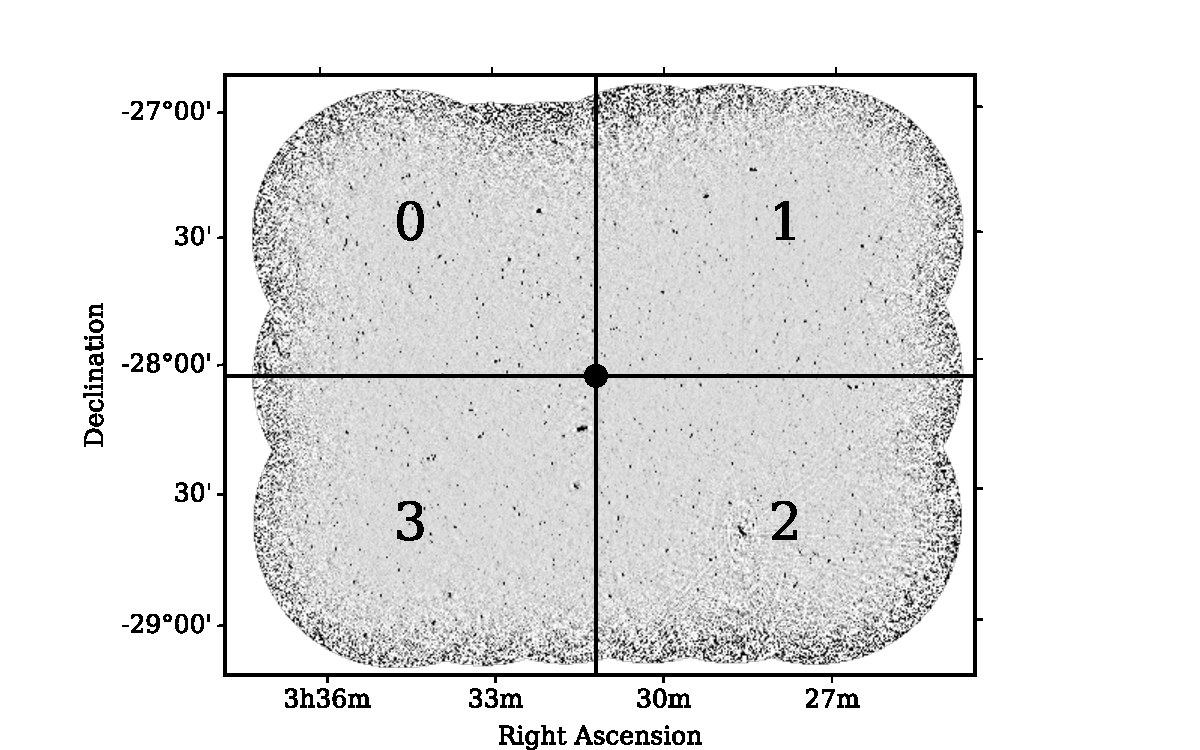
\includegraphics[width=\columnwidth]{images/quadrants.pdf}
      \caption{CDFS field training and testing quadrants labelled 0 -- 3. The
        central dot is located at $\alpha = 03^\text{h}31^\text{m}12^\text{s},
        \delta = -28^\circ{}06'00''$. The quadrants were chosen such that
        there are similar numbers of radio sources in each
        quadrant.\label{fig:quadrants}}
    \end{figure}

    \begin{table}
      \caption{Number of compact and resolved radio objects in each CDFS
      quadrant. Radio Galaxy Zoo (RGZ) has more cross-identifications than the
      expert catalogue provides as it uses a deeper data release of ATLAS, and
      so has more objects in each quadrant for training.}
      \label{tab:radio-count}
      \begin{tabular}{lcccc}
        \hline
        Quadrant & Compact & Resolved & Compact & Resolved\\
        &&&(RGZ)&(RGZ)\\
        \hline
        0 & 126 & 24 & 410 & 43 \\
        1 & 99 & 21 & 659 & 54 \\
        2 & 61 & 24 & 555 & 57 \\
        3 & 95 & 18 & 631 & 51 \\
        \hline
        \textit{Total} & 381 & 87 & 2255 & 205\\
        \hline
      \end{tabular}
    \end{table}

    \begin{figure}
      \centering
      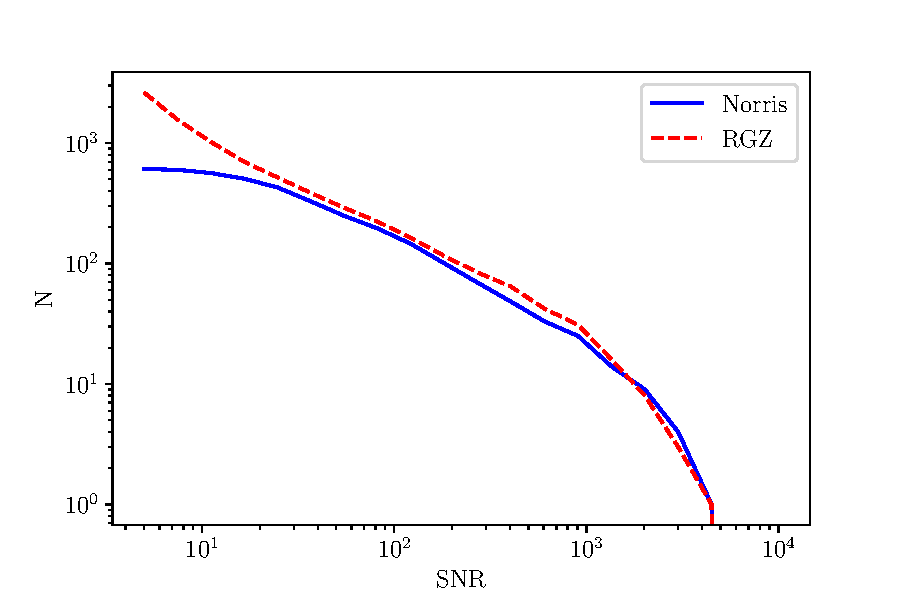
\includegraphics[width=\columnwidth]{images/snr_cutoff_cumulative.pdf}
      \caption{Number of radio components ($N$) in the expert (Norris) and Radio Galaxy
        Zoo (RGZ) training sets with different signal-to-noise (SNR) cutoffs.}
      \label{fig:distribution-cutoffs}
    \end{figure}

    \edited{The Radio Galaxy Zoo and \citet{norris06} cross-identification
    catalogues must be converted to binary labels for infrared objects so that
    they can be used to train binary classifiers.} One problem is that there is
    no clear way to capture radio morphology information in binary
    classification of infrared objects. Another problem is that there is no
    way to indicate \emph{which} radio object an infrared object is associated
    with, only that it is associated with \emph{some} radio object. We ignore
    these problems for this paper and make the na\"ive assumption that any
    given search radius contains only one host galaxy. This allows us to
    assume that if a candidate host galaxy in the search radius of a component
    is not the host galaxy of that component, then it is not a host galaxy at
    all. This is not ideal as it discards information about whether a
    candidate host is not a host galaxy, or whether it was just not
    acknowledged as a host galaxy in the catalogue, but this ambiguity can be
    treated as a source of label noise and will not strongly affect training.

    We then generate positive labels from a cross-identification catalogue.
    We decide that if an infrared object is listed in the catalogue, then it
    is assigned a positive label as a host galaxy. We then assign every other galaxy a negative label. This has some problems
    --- an example is that if the catalogue did not include a radio
    object (e.g.~it was below the signal-to-noise ratio) then the host galaxy
    of that radio object would receive a negative label. This occurs with
    \citet{norris06} cross-identifications, as these are associated with the
    first data release of ATLAS. The first data release went to a 5$\sigma$
    flux density level of $S_{1.4} \geq \unit{200}{\micro\jansky}\text{
    beam}^{-1}$ \citep{norris06}, compared to $S_{1.4} \geq \unit{85}{\micro\jansky}\text{
    beam}^{-1}$ for the third data release used by Radio Galaxy Zoo
    \citep{franzen15}. The labels from \citet{norris06} may therefore disagree with labels
    from Radio Galaxy Zoo even if they are both plausible. The difference in
    training set size at different flux cutoffs is shown in
    \autoref{fig:distribution-cutoffs}. We train and test our binary
    classifiers on infrared objects within a 1~arcmin radius of an ATLAS radio
    object.

  \subsection{Experimental Setup}
  \label{sec:experimental-setup}

    We trained binary classifiers on infrared objects in the CDFS field using
    two sets of labels. One label set was derived from Radio Galaxy Zoo
    cross-identifications and the other was derived from the \citet{norris06}
    cross-identification catalogue. We refer to these as the `Radio Galaxy Zoo
    labels' and the `expert labels' respectively. We divided the CDFS field
    into four quadrants for training and testing. The quadrants were divided
    with a common corner at $\alpha = 03^\text{h}31^\text{m}12^\text{s},
    \delta = -28^\circ{}06'00''$ as shown in \autoref{fig:quadrants}. For
    each trial, one quadrant was used to draw test examples and the other
    three quadrants were used for training examples.

    We further divided the radio components into compact and resolved. Compact
    components are cross-identified by fitting a 2D Gaussian \citep[as
    in][]{norris06} and we would expect any machine learning approach for host
    cross-identification to attain high accuracy on this set. A radio component was
    considered resolved if
    \begin{equation}
        \ln \left(
          \frac{S_{\text{int}}}
               {S_{\text{peak}}}
        \right) > 2\sqrt{\left(
          \frac{\sigma_{S_{\text{int}}}}
               {S_{\text{int}}}
        \right)^2 + \left(
          \frac{\sigma_{S_{\text{peak}}}}
               {S_{\text{peak}}}
        \right)^2}\,\,\,\,,
    \end{equation}%
    where \(S_{\text{int}}\) is the integrated flux density,
    \(S_{\text{peak}}\) is the peak flux density, \edited{$\sigma_{S_{\text{int}}}$ is
    the uncertainty in integrated flux density and $\sigma_{S_{\text{peak}}}$
    is the uncertainty in peak flux density} \citep[following][]{franzen15}.

    Candidate hosts were selected from the SWIRE catalogue. For a given subset
    of radio components, all SWIRE objects within 1~arcmin of all radio
    components in the subset were added to the associated SWIRE subset. In the
    context of the galaxy classification task, we refer to SWIRE objects
    within 1~arcmin of a compact radio component as part of the `compact set',
    and SWIRE objects within 1~arcmin of a resolved radio component as part of
    the `resolved set'.

    To reduce bias in the testing data due to the expert labels being
    generated from a shallower data release of ATLAS, a SWIRE object was only
    included in the test set if it was within 1~arcmin of a radio object with
    a cross-identification in both the \citet{norris06} catalogue and the
    Radio Galaxy Zoo catalogue.

    Each binary classifier was trained on the training examples and used to
    predict labels for the test examples. The predicted labels were compared
    to the expert labels and the balanced accuracy was computed. Balanced
    accuracy is the average of the accuracy on the positive class and the
    accuracy on the negative class, and is not sensitive to class imbalance.
    The galaxy classification task has highly imbalanced classes --- in our
    total set of SWIRE objects within 1~arcmin of an ATLAS object, only 4~per
    cent have positive labels. Only examples within 1~arcmin of ATLAS objects
    in the first ATLAS data release \citep{norris06} were used to compute
    accuracy, as these were the only ATLAS objects with expert labels.

    We then used the estimated class probabilities to predict the host galaxy
    for each radio component cross-identified by both \citet{norris06} and
    Radio Galaxy Zoo. For each SWIRE object within 1~arcmin of the radio
    component, the probability of the object having a positive label was
    estimated using the trained binary classifiers. The SWIRE object with the
    highest Gaussian-weighted probability was chosen as the host galaxy. The
    accuracy for the cross-identification task was then estimated as the
    fraction of the predicted host galaxies that matched the \citet{norris06}
    cross-identifications.

\section{Results}\label{sec:results}

  In this section we present accuracies of our method trained on CDFS and
  applied to CDFS and ELAIS-S1, as well as results motivating our accuracy
  measures and estimates of upper and lower bounds for cross-identification
  accuracy using our method.

  \subsection{Application to ATLAS-CDFS}
  \label{sec:cdfs-results}

    \begin{figure}
      \centering
      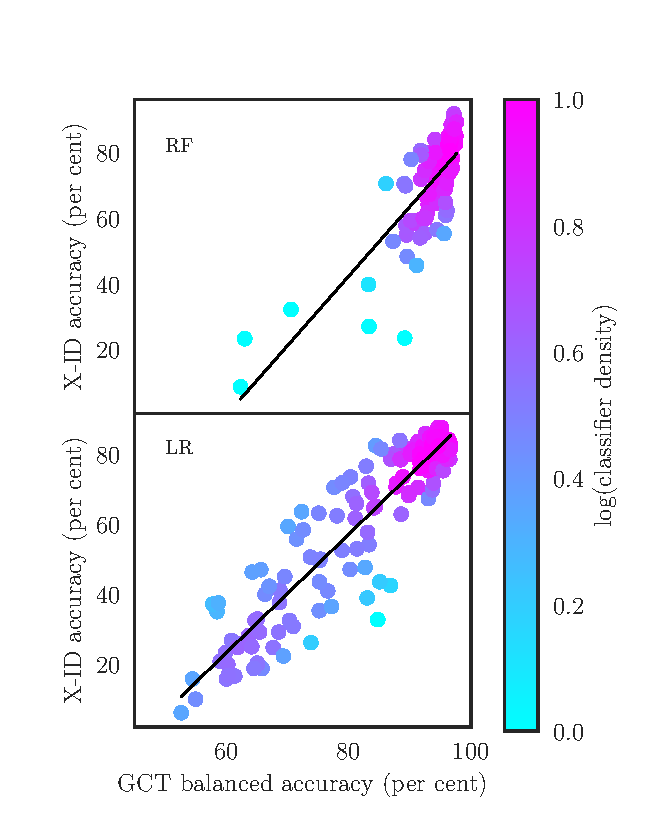
\includegraphics[width=\columnwidth]{images/gct-to-xid.pdf}
      \caption{Balanced accuracy on the galaxy classification task (GCT) plotted
      against accuracy on the cross-identification task (X-ID). RF indicates
      results from random forests, and LR indicates results from logistic
      regression. Binary classifiers were trained on random, small subsets of the
      training data to artificially restrict their accuracies. Colour shows
      the density of points on the plot estimated by a Gaussian kernel density
      estimate. The solid lines indicate the best linear fit; these fits have
      $R^2 = 0.92$ for logistic regression and $R^2 = 0.87$ for random
      forests. We did not include convolutional neural networks in this test,
      as training them is very computationally expensive. There are 640 trials shown per classification model. These results
      exclude binary classifiers with balanced accuracies less than 51 per cent, as
      these are essentially random.
      \label{fig:gct-to-xid}}
    \end{figure}

    \begin{figure}
      \centering
      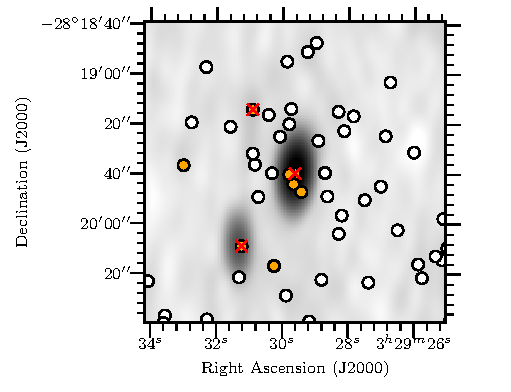
\includegraphics[width=\columnwidth]{images/positives.pdf}
      \caption{ATLAS3~J032929.61-281938.9. Radio Galaxy Zoo host galaxies are marked by crosses. SWIRE candidate host galaxies are circles, coloured orange circles have been assigned a `positive' label by a logistic regression binary classifier and white otherwise.
      \label{fig:positives}}
    \end{figure}

    \begin{figure}
    \centering
    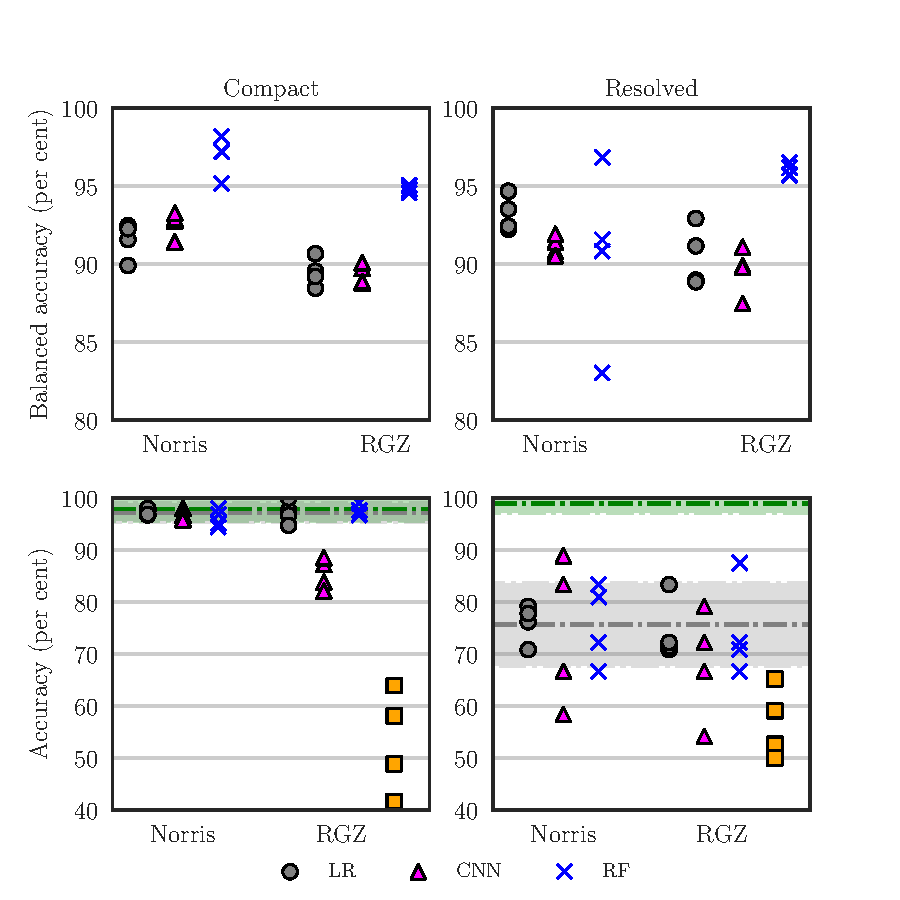
\includegraphics[width=\columnwidth]{images/cdfs-grid-new.pdf}
    \caption{Performance of our method with logistic regression (LR), convolutional neural networks (CNN) and random forest (RF) binary classifiers. `Norris' indicates the performance of binary classifiers trained on the expert labels and `RGZ' indicates the performance of binary classifiers trained on the Radio Galaxy Zoo labels. One point is shown per binary classifier per testing quadrant. The training and testing sets have been split into compact and resolved objects, with results on compact objects shown on the left and results on resolved objects shown on the right. \edited{Shown for comparison is the accuracy of the Radio Galaxy Zoo consensus cross-identifications on the cross-identification task, shown as `Labels'.} The cross-identification accuracy attained by a perfect binary classifier is shown by a solid green line, and the cross-identification accuracy of a nearest-neighbours approach is shown by a dashed grey line. The standard deviation of these accuracies across the four CDFS quadrants is shown by the shaded area. Note that the pipeline shown in \autoref{fig:flowchart} is not used for these results. \label{fig:ba}}
    \end{figure}

    \begin{figure}
      \centering
      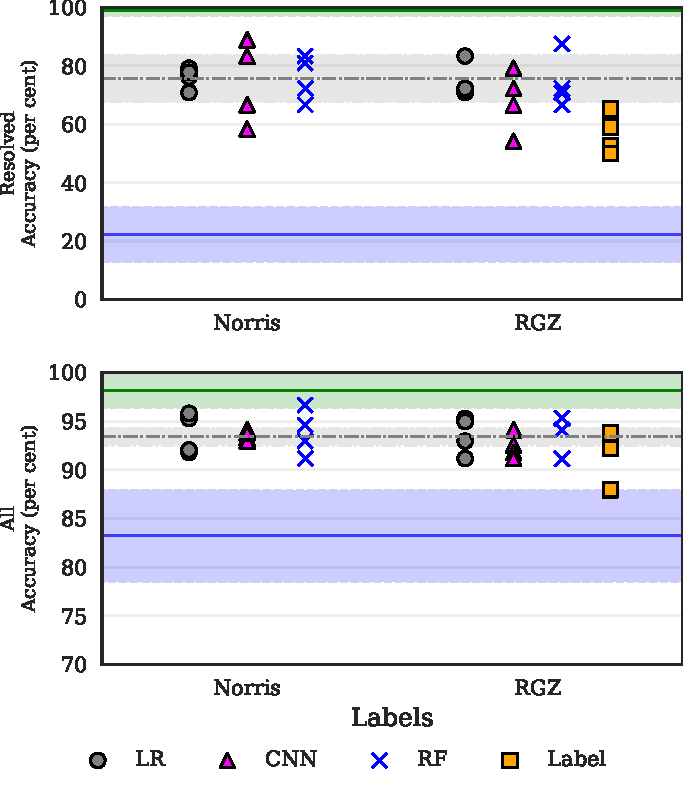
\includegraphics[width=0.9\columnwidth]{images/cdfs_cross_identification_grid.pdf}
      \caption{Performance of our approach using different binary classifiers on the cross-identification task. Markers and lines are as in \autoref{fig:ba}. The blue solid line indicates the performance of a random binary classifier and represents the minimum accuracy we expect to obtain. The standard deviation of this accuracy across 25 trials and 4 quadrants is shaded. The accuracy of Radio Galaxy Zoo on the cross-identification task is below the axis and is instead marked by an arrow with the mean accuracy. Note that the pipeline shown in \autoref{fig:flowchart} is used here, \edited{so compact objects are cross-identified in the same way regardless of binary classifier model}. \label{fig:cross-id-accuracy}}
    \end{figure}

    \begin{figure*}
        \subfloat[]{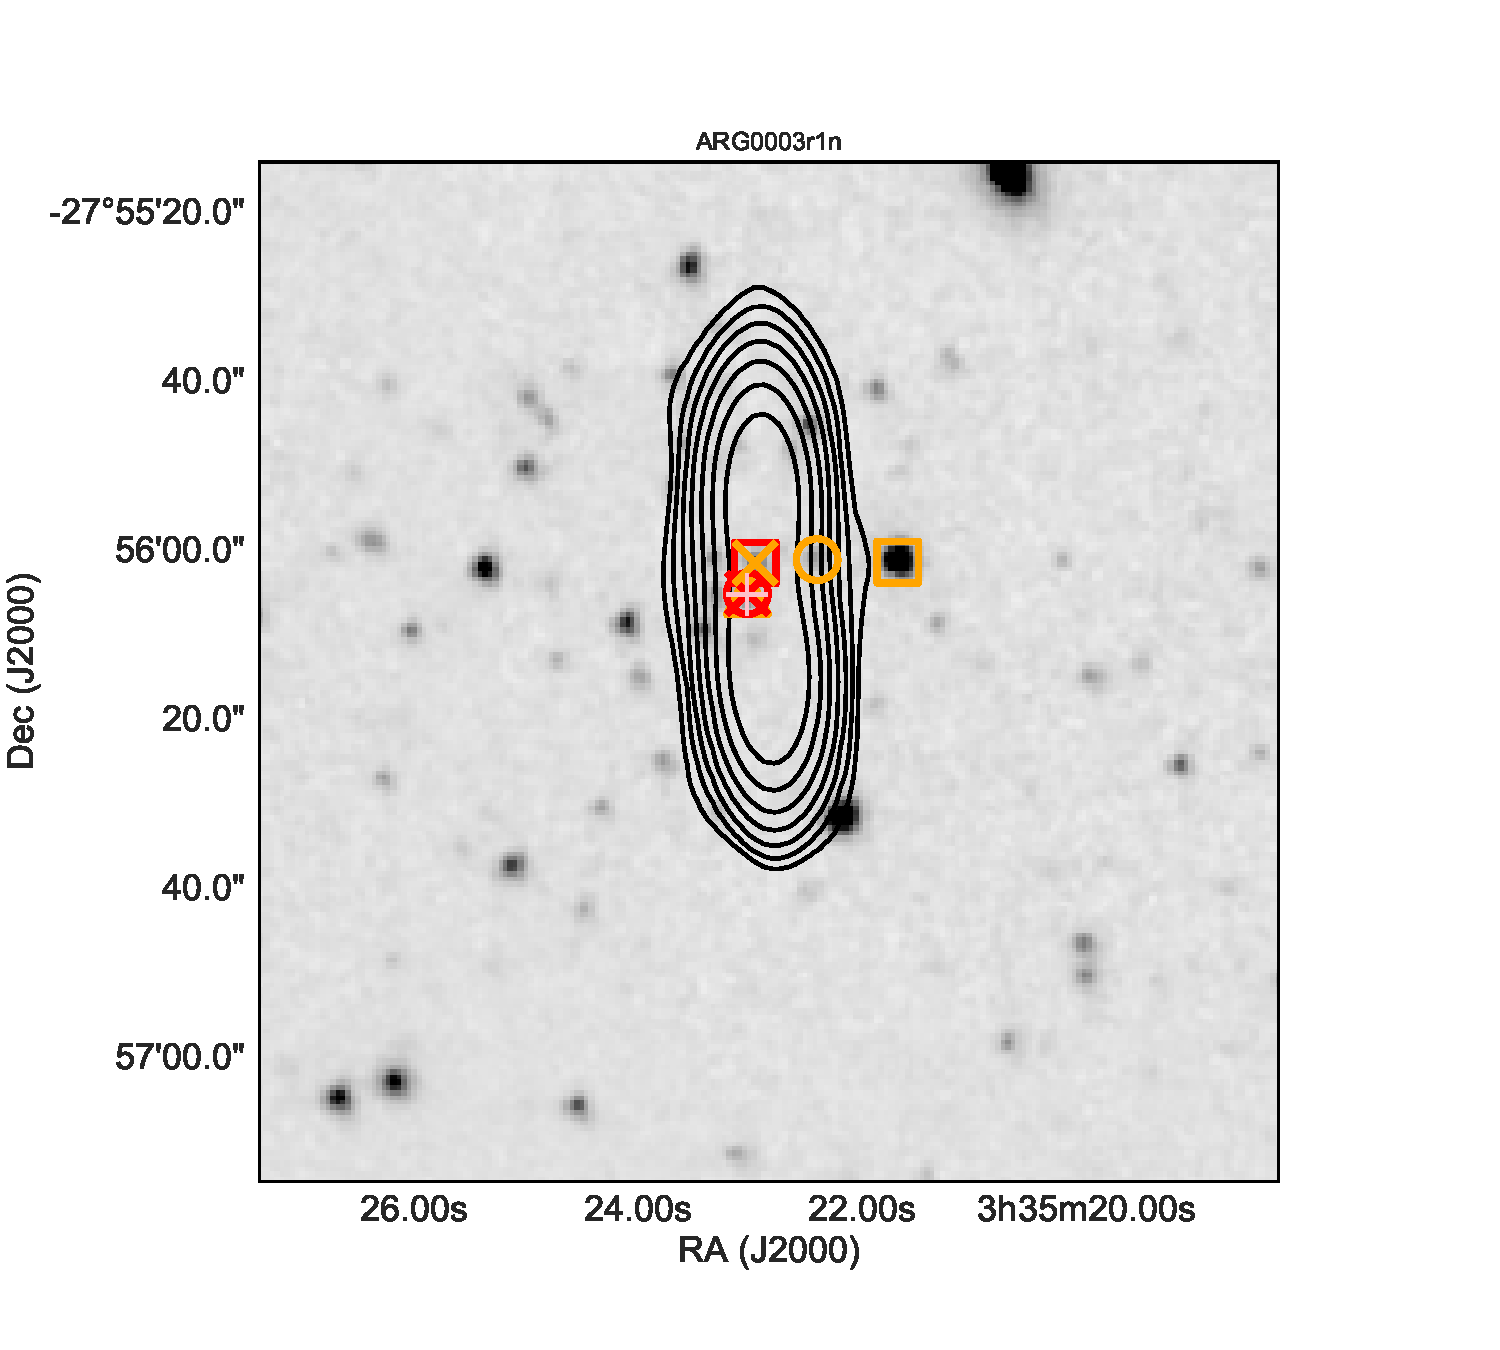
\includegraphics[trim={0cm 1cm 3.5cm 2.6cm}, clip, width=0.33\textwidth]{images/example_15_454.pdf}}%
        \subfloat[]{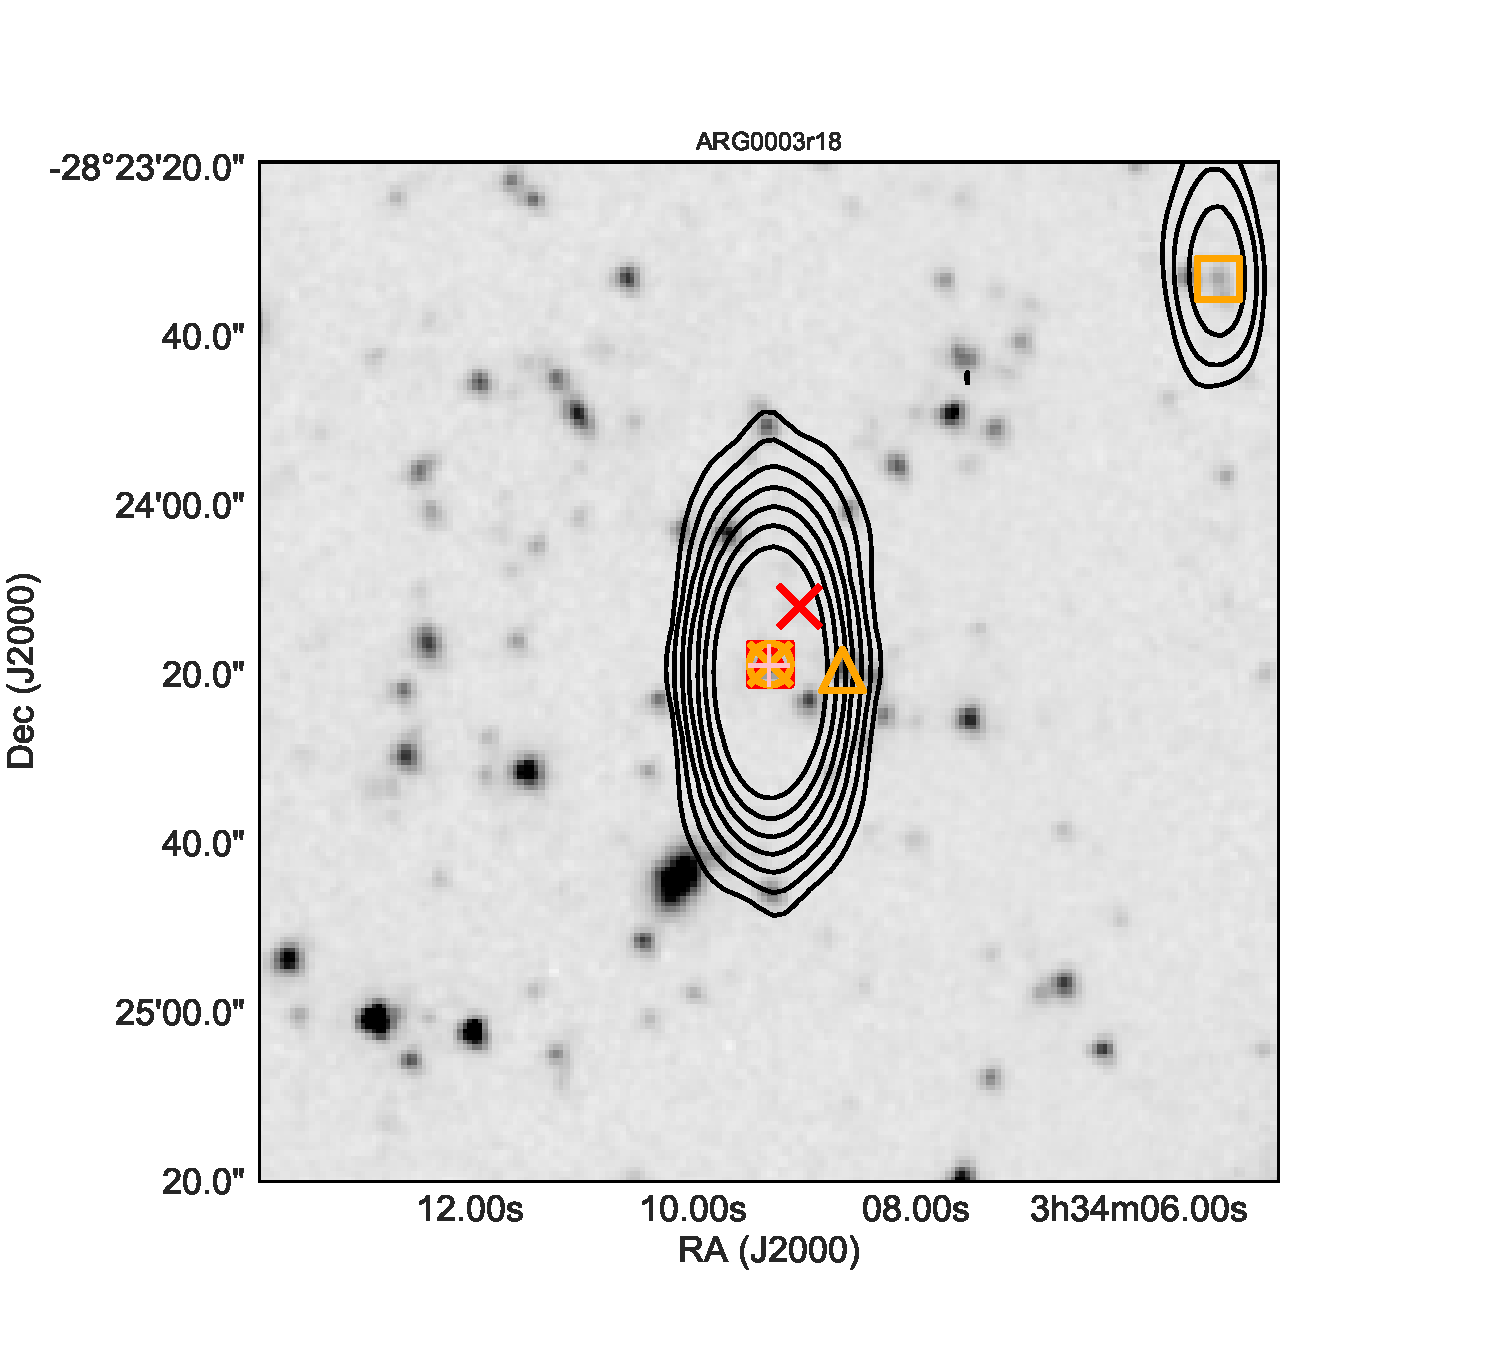
\includegraphics[trim={0cm 1cm 3.5cm 2.6cm}, clip, width=0.33\textwidth]{images/example_12_404.pdf}}%
        \subfloat[]{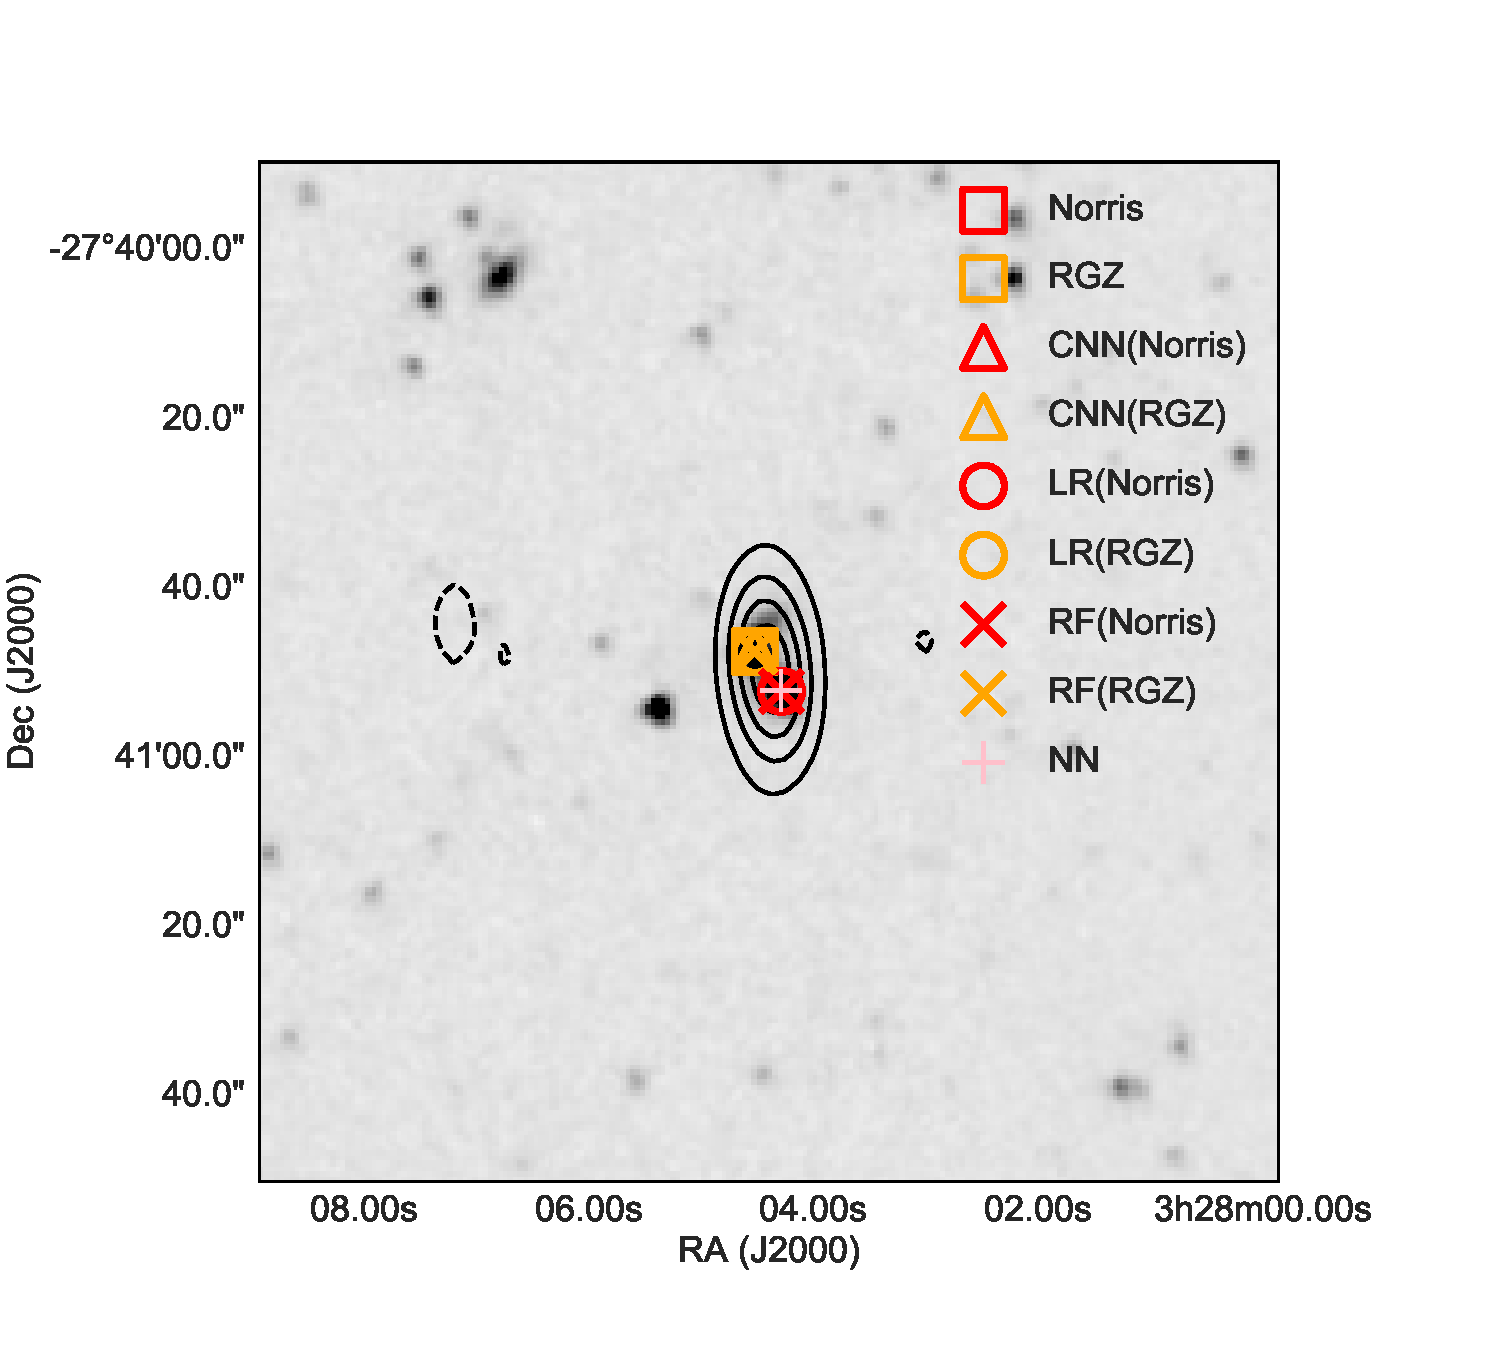
\includegraphics[trim={0cm 1cm 3.5cm 2.6cm}, clip, width=0.33\textwidth]{images/example_2_68.pdf}}

        \subfloat[]{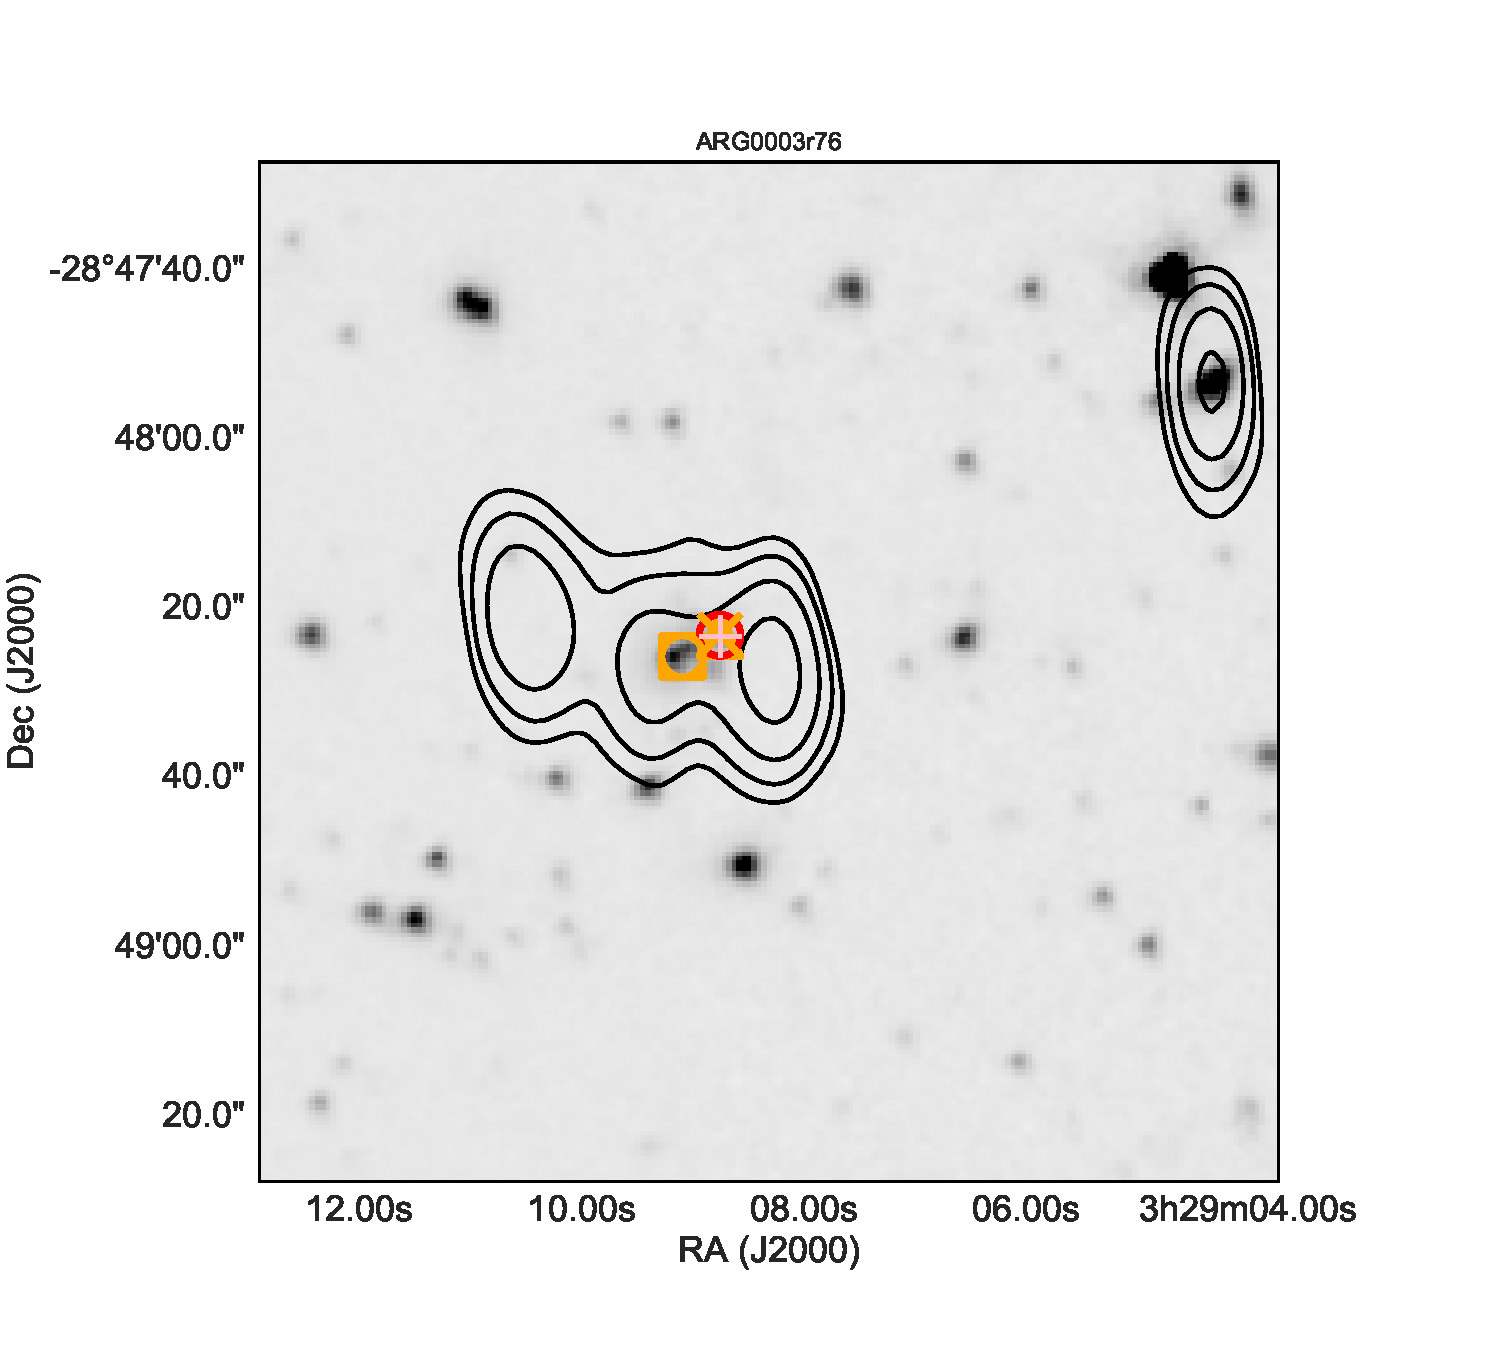
\includegraphics[trim={0cm 1cm 3.5cm 2.6cm}, clip, width=0.33\textwidth]{images/example_4_106.pdf}}%
        \subfloat[]{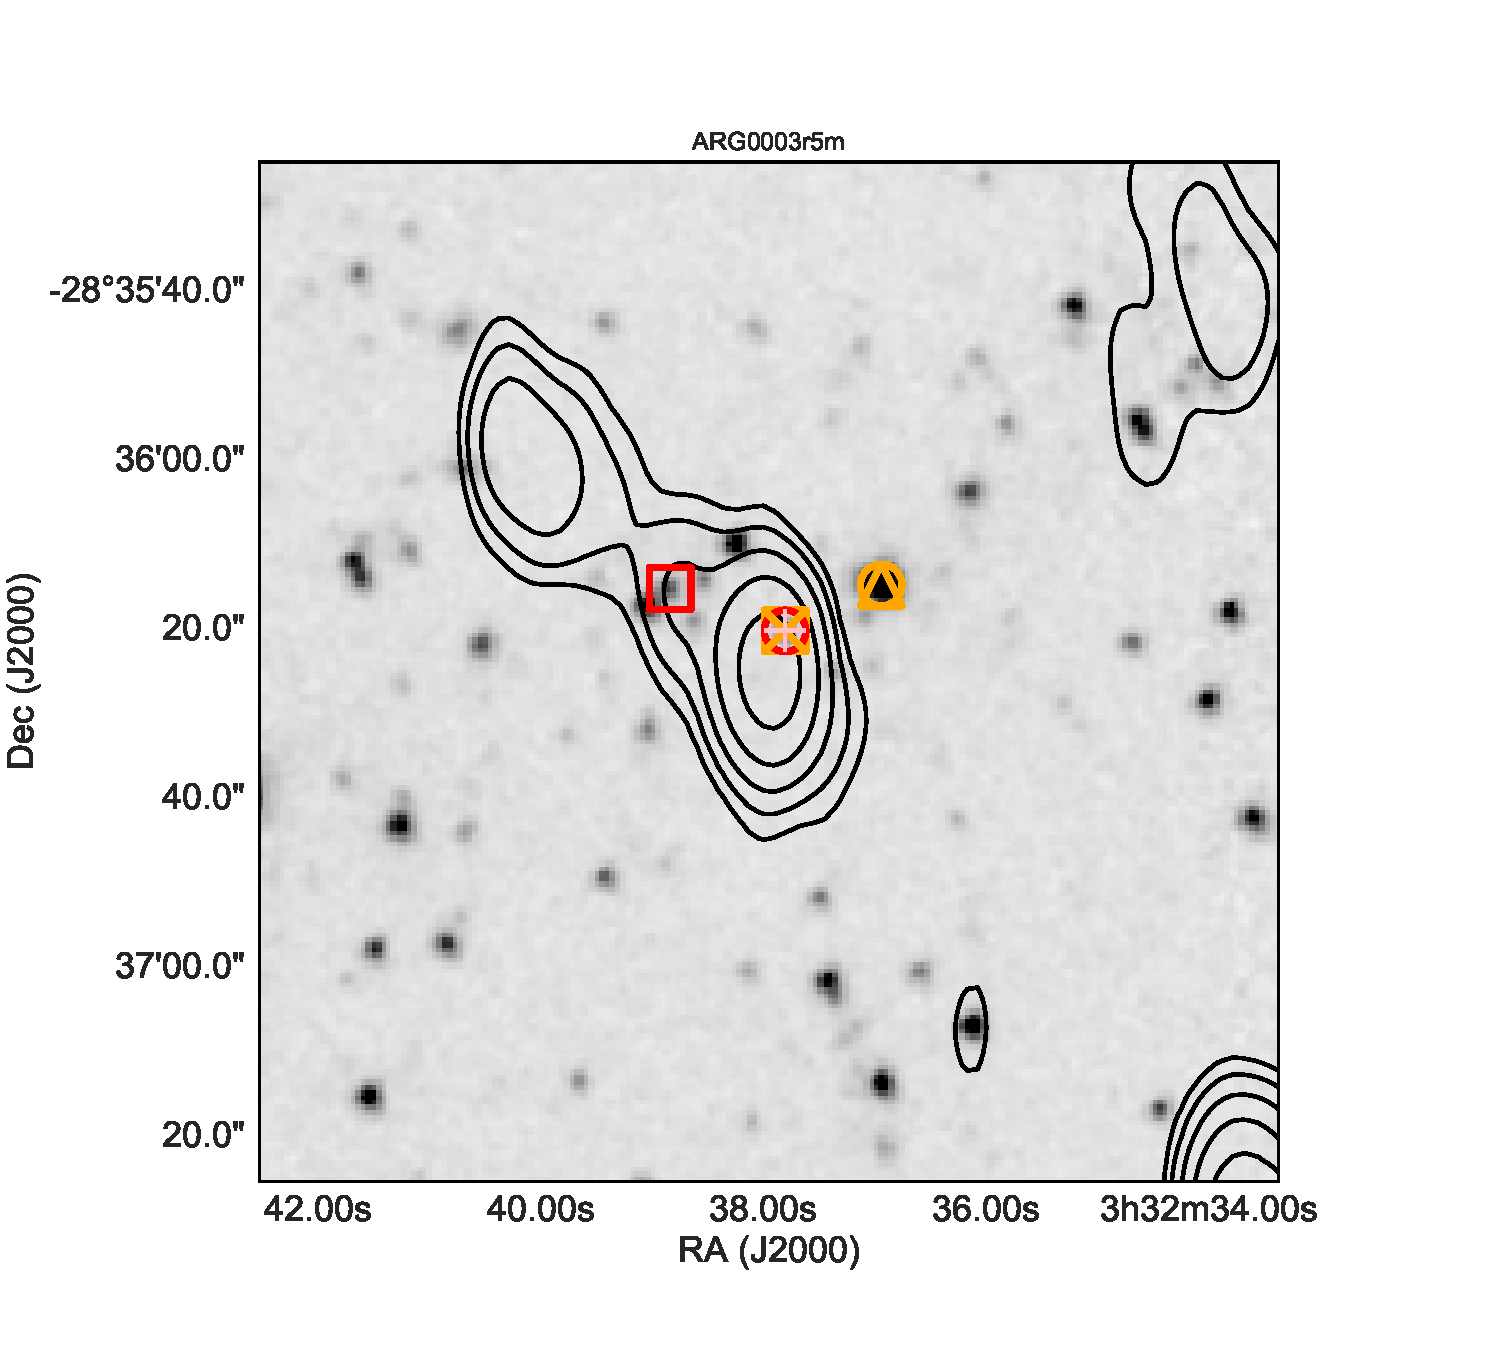
\includegraphics[trim={0cm 1cm 3.5cm 2.6cm}, clip, width=0.33\textwidth]{images/example_10_298.pdf}}%
        \subfloat[]{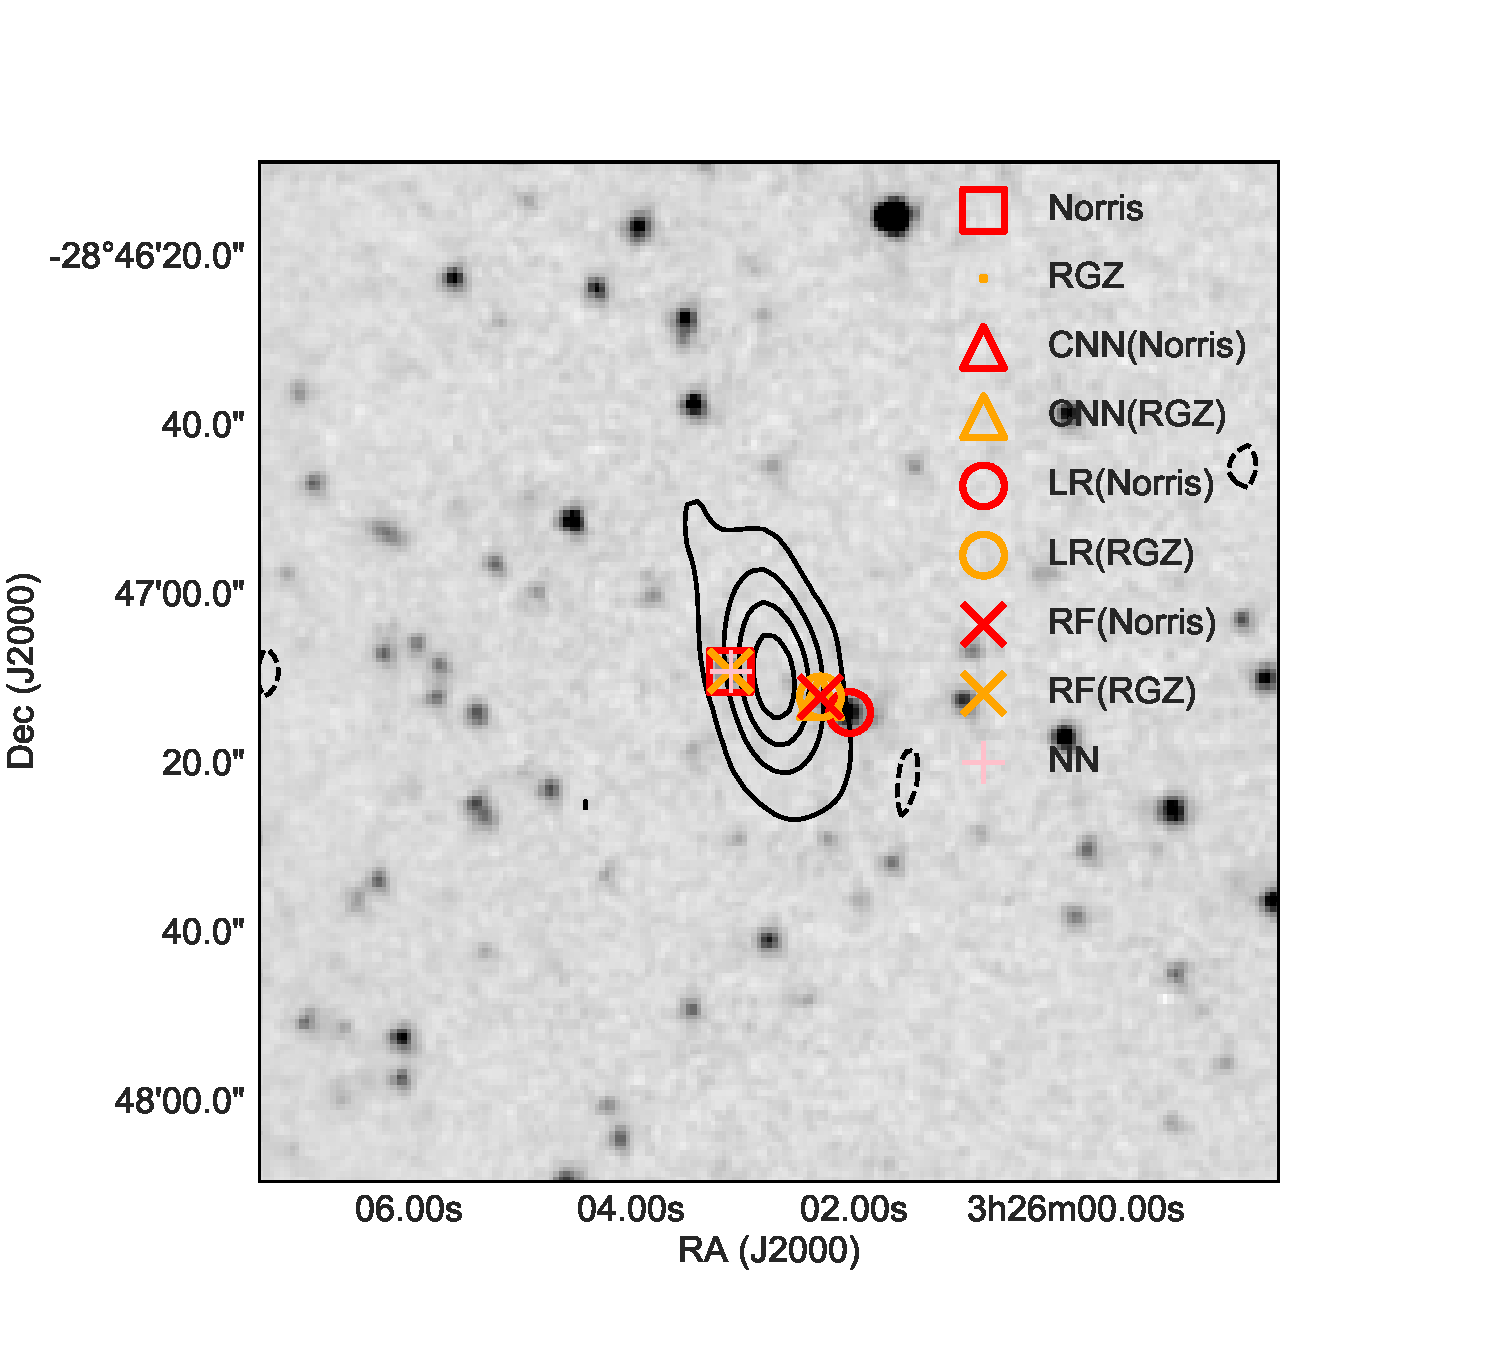
\includegraphics[trim={0cm 1cm 3.5cm 2.6cm}, clip, width=0.33\textwidth]{images/example_0_0.pdf}}%
        \caption{\label{fig:examples} Examples of resolved sources where the incorrect cross-identification was selected by random forests trained on expert labels. Binary classifier model/training set combinations are denoted $C(S)$ where $C$ is the binary classifier model and $S$ is the training set. `LR' is logistic regression, `CNN' is convolutional neural networks, and `RF' is random forests. `Norris' refers to the expert labels and `RGZ' refers to the Radio Galaxy Zoo labels. The cross-identification made by nearest-neighbours is shown by `NN'. The background image is the \unit{3.6}{\micro\meter} SWIRE image. The contours show ATLAS radio data and increase geometrically from a signal-to-noise ratio of 4.}
    \end{figure*}

    \edited{We can assess trained binary classifiers either by their performance on
    the galaxy classification task or by their performance on the
    cross-identification task when used in our method. Both performances are
    useful: performance on the galaxy classification task provides a robust
    and simple way to compare binary classifiers without the limitations of
    our specific formulation, and performance on the cross-identification task
    can be compared with other cross-identification methods. We therefore
    report two sets of accuracies: balanced accuracy for the galaxy
    classification task and accuracy for the cross-identification task. These
    accuracy measures are correlated and we show this correlation in
    \autoref{fig:gct-to-xid}. Fitting a line of best fit with \texttt{scipy}
    gives $R^2 = 0.92$ for logistic regression and $R^2 = 0.87$ for random
    forests. While performance on the galaxy classification task is correlated
    with performance on the cross-identification task, balanced accuracy does
    not completely capture the effectiveness of a binary classifier applied to
    the cross-identification task. \edited{This is because while our binary
    classifiers output probabilities, these probabilities are thresholded to
    compute the balanced accuracy}. In the galaxy classification
    task, the binary classifier only needs to ensure that host galaxies are
    given higher probabilities than non-host galaxies. This means there can be
    many `false positives' that do not affect cross-identification. An example
    of this is shown in \autoref{fig:positives}, where the classifier has
    identified 8 `host galaxies'. However, there are only three true host
    galaxies in this image --- one per radio component --- and so in the
    cross-identification task, only three of these galaxies will be identified
    as hosts.}

    In \autoref{fig:ba} we plot the performance of logistic regression, random
    forests, and a convolutional neural network on both the galaxy
    classification task and the cross-identification task for resolved and
    compact sources. For comparison, we also plot the accuracy of Radio Galaxy
    Zoo and a nearest-neighbours approach, as well as estimates for upper and
    lower limits on the cross-identification accuracy. \edited{We estimate the upper limit on performance by assigning all
    true host galaxies a 100 per cent probability of being host galaxies and
    assigning all other candidate host galaxies a 0 per cent probability. This
    is equivalent to `perfectly' solving the galaxy classification task and so
    represents the best possible cross-identification performance achievable
    with our method. We estimate the lower limit on performance by taking a
    random binary classifier, which outputs random probabilities regardless of
    input galaxy. We expect any useful binary classifier to produce better
    results than this, so this represents the lowest expected
    cross-identification performance.} The upper estimates, lower estimates,
    and nearest-neighbour accuracy are shown as horizontal lines in
    \autoref{fig:ba}.

    In \autoref{fig:cross-id-accuracy} we plot the performance \edited{of our
    method with different binary classification models}, as well as the
    performance of Radio Galaxy Zoo, nearest-neighbours, and the perfect and
    random binary classifiers, on the full set of ATLAS~DR1 radio components
    using the pipeline in \autoref{fig:flowchart}. The average accuracy
    \edited{associated with each classification model} and training label set
    across all four quadrants is shown in \aref{app:accuracies}.

    Differences between accuracies across training labels are well within one
    standard deviation computed across the four quadrants, with convolutional
    neural networks on compact objects as the only exception. The spread of
    accuracies is similar for both sets of training labels, with the exception
    of random forests. The balanced accuracies of random forests trained on
    expert labels have a considerably higher spread than those trained on
    Radio Galaxy Zoo labels, likely because of the small size of the expert
    training set --- there are less than half the number of objects in the
    expert-labelled training set than the number of objects in the Radio
    Galaxy Zoo-labelled training set (\autoref{tab:radio-count}).

    Radio Galaxy Zoo-trained methods significantly outperform Radio Galaxy Zoo
    cross-identifications. Additionally, despite poor performance of Radio
    Galaxy Zoo on the cross-identification task, methods trained on these
    cross-identifications still perform comparably to those trained on expert
    labels. This is because incorrect Radio Galaxy Zoo cross-identifications
    can be thought of as a source of noise in the labels which is averaged out
    in training. This shows the usefulness of crowdsourced training data, even
    when the data is noisy.

    Our method performs comparably to a nearest-neighbours approach. For
    compact objects, this is to be expected --- indeed, nearest-neighbours
    attains nearly 100 per cent accuracy on the compact test set. Our results
    do not improve on nearest-neighbours for resolved objects. However, our
    method does allow for improvement on nearest-neighbours with a
    sufficiently good binary classifier: a `perfect' binary classifier attains
    nearly 100 per cent accuracy on resolved sources. This shows that our
    method may be useful provided that a good binary classifier can be
    trained. The most obvious place for improvement is in feature selection:
    we use pixels of radio images directly and these are likely not conducive
    to good performance on the galaxy classification task. Convolutional
    neural networks, which are able to extract features from images,
    \emph{should} work better, but these require far more training data than
    the other methods we have applied and the small size of ATLAS thus results
    in poor performance.

    We noted in \autoref{sec:labels} that the test set of expert labels,
    derived from the initial ATLAS data release, was less deep than the third
    data release used by Radio Galaxy Zoo and this paper, introducing a source
    of label noise in the testing labels. Specifically, true host galaxies may
    be misidentified as non-host galaxies if the associated radio source was
    below the 5 signal-to-noise limit in ATLAS DR1 but not in ATLAS DR3. This
    has the effect of reducing the accuracy for Radio Galaxy Zoo-trained
    classifiers.

    \edited{We report the probabilities predicted by each classifier for each
    SWIRE object in \aref{app:probabilities} and the predicted
    cross-identification for each ATLAS object in \aref{app:xids}.
    Probabilities reported for a given object were predicted by binary
    classifiers tested on the quadrant containing that object.}

    In \autoref{fig:examples} we show 6 of the 16 resolved sources where the
    incorrect cross-identification was selected by random forests trained on
    expert labels. The remaining 10 sources are shown in \aref{app:examples}.
    In most cases the incorrect galaxy selected was also selected by
    nearest-neighbours. We note that on no source do all classifiers agree.
    This raises the possibility of using the level of disagreement of an
    ensemble of classifiers as a measure of the complexity of a radio source,
    analogous to the consensus level for Radio Galaxy Zoo volunteers.

\subsection{Application to ATLAS-ELAIS-S1}
  \label{sec:elais}

  \begin{figure}
  \centering
  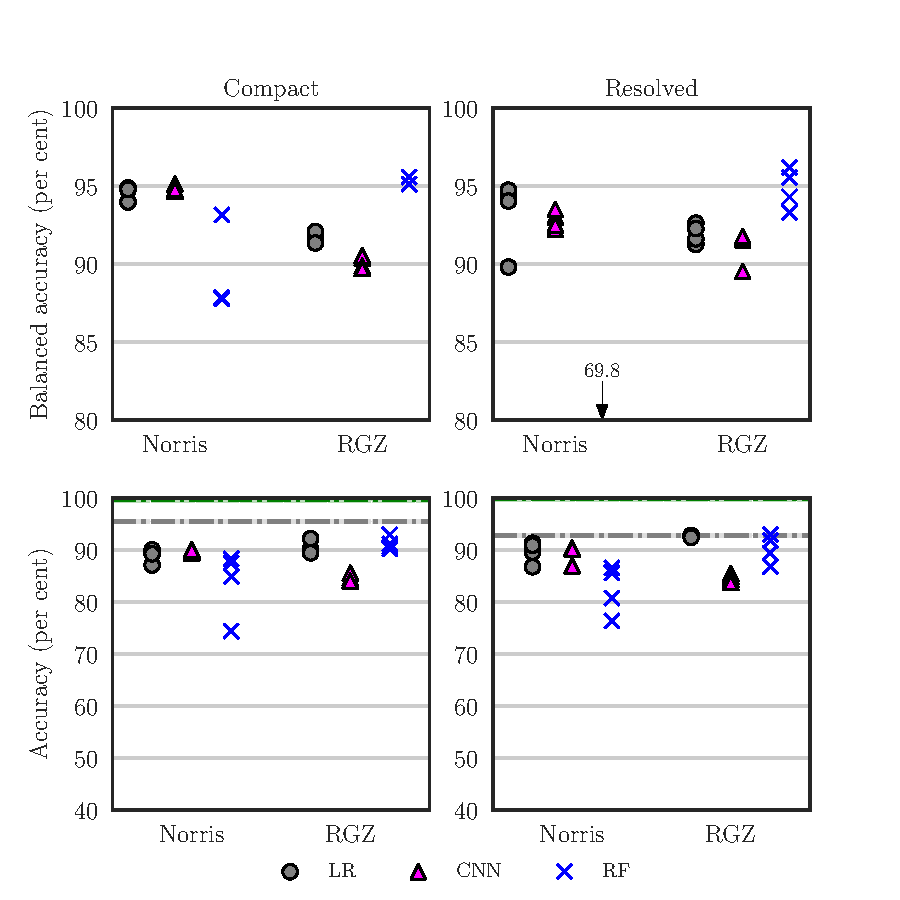
\includegraphics[width=\columnwidth]{images/elais-grid-new.pdf}
  \caption{Performance of different classifiers trained on CDFS and tested on
  resolved and compact sources in ELAIS-S1. Points represent classifiers
  trained on different quadrants of CDFS, with markers and axes as in
  \autoref{fig:ba}. The balanced acccuracy of expert-trained random forest
  classifiers falls below the axis and the corresponding mean accuracy is
  shown by an arrow. The solid green line indicates the cross-identification
  accuracy of a `perfect' classifier; this is almost 100 per cent. The grey
  dashed line indicates the cross-identification accuracy of
  nearest-neighbours.
    \label{fig:elais-ba}}
  \end{figure}

  \begin{figure}
    \centering
    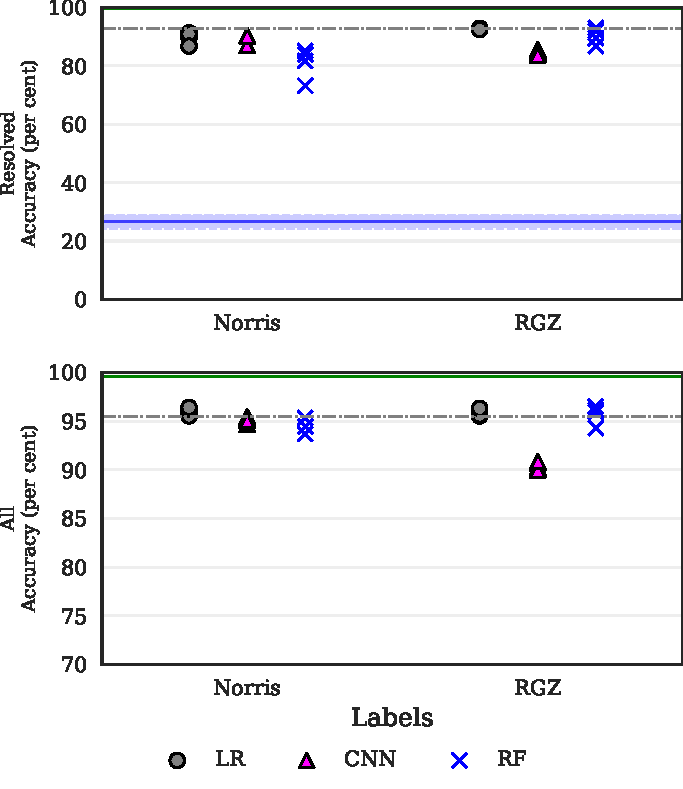
\includegraphics[width=0.9\columnwidth]{images/elais_cross_identification_grid.pdf}
    \caption{Performance of different classifiers trained on CDFS and tested
    on ELAIS-S1. Markers are as in \autoref{fig:cross-id-accuracy} and
    horizontal lines are as in \autoref{fig:elais-ba}. Note that the pipeline
    shown in \autoref{fig:flowchart} is used here, \edited{so compact objects
    are cross-identified in the same way regardless of binary classifier
    model}.
      \label{fig:elais-cross-id-accuracy}}
  \end{figure}

  \begin{figure}
    \centering
    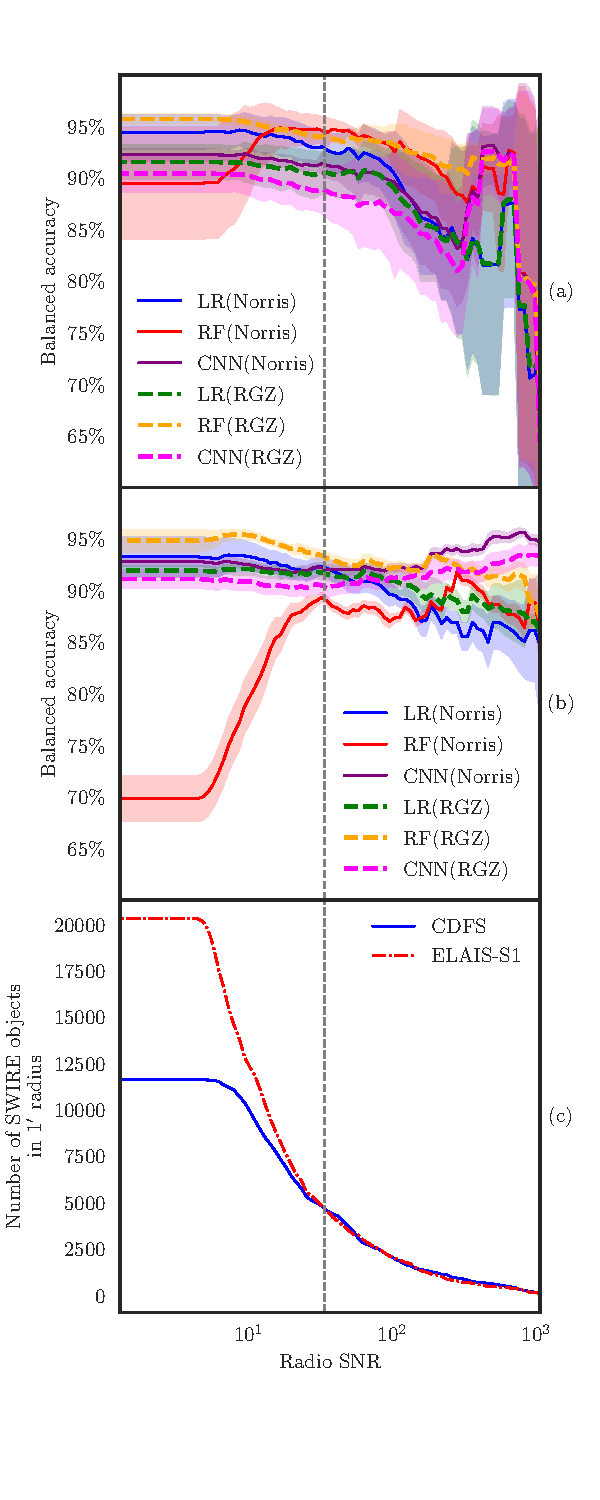
\includegraphics[width=\columnwidth, clip,
                     trim={0 2cm 0 1cm}]{images/accuracies-flux-snr.pdf}
    \caption{(a) Balanced accuracies of classifiers trained and tested on CDFS
      with different signal-to-noise ratio (SNR) cutoffs for the test set. A
      SWIRE object is included in the test set if it is within $1'$ of a radio
      component with greater SNR than the cutoff. Different coloured lines
      indicate different classifier/training labels combinations, where LR is
      logistic regression, RF is random forests, CNN is convolutional neural
      networks, and Norris and RGZ are the expert and Radio Galaxy Zoo label
      sets respectively. Filled areas represent standard deviations across
      CDFS quadrants. (b) Balanced accuracies of classifiers trained on CDFS
      and tested on ELAIS-S1. (c) A cumulative distribution plot of SWIRE
      objects associated with a radio object with greater SNR than the cutoff.
      The grey dashed line shows the SNR level at which the number of SWIRE
      objects above the cutoff is equal for CDFS and ELAIS-S1. This cutoff level
      is approximately $34$ times the RMS.}
    \label{fig:accuracies-flux}
  \end{figure}

  We applied the method trained on CDFS to perform cross-identification on the
  ELAIS-S1 field. Both CDFS and ELAIS-S1 were imaged by the same radio
  telescope to similar sensitivities and angular resolution for the ATLAS
  survey. \edited{We can use the SWIRE cross-identifications made by
  \citet{middelberg08} to derive another set of expert labels, and hence
  determine how accurate our method is. If our method generalises well across
  different parts of the sky, then we expect CDFS-trained classifiers to have
  comparable performance between ELAIS-S1 and CDFS}. In \autoref{fig:elais-ba}
  we plot the performance of CDFS-trained logistic regression, random forests,
  and convolutional neural networks on both the galaxy classification task and
  the cross-identification task for resolved and compact sources. We also plot
  the accuracy of a nearest-neighbours approach\footnote{\edited{We cannot
  directly compare our method applied to ELAIS-S1 with Radio Galaxy Zoo, as
  Radio Galaxy Zoo does not include ELAIS-S1.}}. In
  \autoref{fig:elais-cross-id-accuracy} we plot the performance of our method
  on the full set of ELAIS-S1 ATLAS~DR1 radio components using the pipeline in
  \autoref{fig:flowchart}. We list the corresponding accuracies in
  \aref{app:accuracies}.

  Cross-identification results from ELAIS-S1 are similar to those for CDFS,
  showing that our method trained on CDFS performs comparably well on
  ELAIS-S1. However, nearest-neighbours outperforms most methods on ELAIS-S1.
  This is likely because there is a much higher percentage of compact objects
  in ELAIS-S1 than in CDFS. The maximum achievable accuracy we have estimated
  for ELAIS-S1 is very close to 100 per cent, so (as for CDFS) a very accurate
  binary classifier would outperform nearest-neighbours.

  One interesting difference between the ATLAS fields is that random forests
  trained on expert labels perform well on CDFS but poorly on ELAIS-S1. This
  is not the case for logistic regression or convolutional neural networks
  trained on expert labels, nor is it the case for random forests trained on
  Radio Galaxy Zoo. We hypothesise that this is because the ELAIS-S1
  cross-identification catalogue \citep{middelberg08} labelled fainter radio
  components than the CDFS cross-identification catalogue \citep{norris06} due
  to noise from the very bright source
  ATCDFS\textunderscore{}J032836.53-284156.0 in CDFS. Classifiers trained on
  CDFS expert labels may thus be biased toward brighter radio components
  compared to ELAIS-S1. Radio Galaxy Zoo uses the third data release of ATLAS
  \citep{franzen15} and so classifiers trained on the Radio Galaxy Zoo labels
  may be less biased toward brighter sources compared to those trained on the
  expert labels. To test this hypothesis we tested each classifier against
  test sets with a signal-to-noise ratio (SNR) cutoff. A SWIRE object was only
  included in the test set for a given cutoff if it was located within $1'$ of
  a radio component with a SNR above the cutoff. The balanced accuracies for
  each classifier at each cutoff are shown in \autoref{fig:accuracies-flux}(a)
  and (b) and the distribution of test set size for each cutoff is shown in
  \autoref{fig:accuracies-flux}(c). \autoref{fig:accuracies-flux}(c) shows
  that ELAIS-S1 indeed has more faint objects than CDFS, with the SNR for
  which the two fields reach the same test set size (approximately $34$)
  indicated by the dashed vertical line on each plot. For CDFS, all
  classifiers perform reasonably well across cutoffs, with performance
  dropping as the size of the test set becomes small. For ELAIS-S1, logistic
  regression and convolutional neural networks perform comparably across all
  SNR cutoffs, but random forests do not. While random forests trained on
  Radio Galaxy Zoo labels perform comparably to other classifiers across all
  SNR cutoffs, random forests trained on expert labels show a considerable
  drop in performance below the dashed line.

\section{Discussion}

  \edited{Based on the ATLAS sample}, our main result is that it is possible
  to cast radio host galaxy cross-identification as a machine learning task
  for which standard methods can be applied. These methods can then be trained
  with a variety of label sets derived from cross-identification catalogues.
  While we have not outperformed nearest-neighbours, we have demonstrated that
  for a very accurate binary classifier, good cross-identification results can
  be obtained using our method. Future work could combine multiple catalogues
  or physical priors to boost performance.

  Nearest-neighbours approaches outperform most methods we investigated,
  notably including Radio Galaxy Zoo. This is due to the large number of
  compact or partially-resolved objects in ATLAS. This result shows that for
  compact and partially-resolved objects methods that do not use machine
  learning such as a nearest-neighbours approach or likelihood ratio
  \citep{weston18lrpy} should be preferred to machine learning methods. It
  also shows that ATLAS is not an ideal data set for developing machine
  learning methods like ours. Our use of ATLAS is motivated by its status as a
  pilot survey for EMU, so methods developed for ATLAS should also work for
  EMU. New methods developed should work well with extended radio sources, but
  this goal is almost unsupported by ATLAS as it has very few examples of such
  sources. This makes both training and testing difficult --- there are too
  few extended sources to train on and performance on such a small test set
  may be unreliable. Larger data sets with many extended sources like FIRST
  exist, but these are considerably less deep than and at a different
  resolution to EMU, so there is no reason to expect methods trained on such
  data sets to be applicable to EMU.

  The accuracies of our trained cross-identification methods generally fall
  far below the best possible accuracy attainable using our approach,
  indicated by the green lines in Figures \ref{fig:cross-id-accuracy} and
  \ref{fig:elais-cross-id-accuracy}. The balanced accuracies attained by our
  binary classifiers indicate that there is significant room for improvement
  in classification. The classification accuracy can be improved by better
  model selection and more training data, particularly for convolutional
  neural networks. There is a huge variety of ways to build a convolutional
  neural network, and we have only investigated one architecture. For an
  exploration of different convolutional neural network architectures applied
  to radio astronomy, see Lukic et al. (in prep). Convolutional neural
  networks generally require more training data than other machine learning
  models and we have only trained our networks on a few hundred sources. We
  would thus expect performance on the classification task to greatly increase
  with larger training sets.

  Another problem is that of the window size used to select radio features.
  Increasing window size would increase computational expense, but provide
  more information to the models. Results are also highly sensitive to how
  large the window size is compared to the size of the radio galaxy we are
  trying to cross-identify, with large angular sizes requiring large window
  sizes to ensure that the features contain all the information needed to
  localise the host galaxy. An ideal implementation of our method would most
  likely represent a galaxy using radio images taken at multiple window
  sizes, but this is considerably more expensive.

  Larger training sets, better model selection, and larger window sizes would
  improve performance, but only so far: we would still be bounded above by the
  estimated ``perfect'' classifier accuracy. From this point, the performance
  can only be improved by improving upon our broken assumptions. We detailed
  these assumptions in \autoref{sec:limitations}, and we will discuss here how
  these could be resolved. Our assumption that the host galaxy is contained
  within the search radius could be improved by dynamically choosing the
  search radius, perhaps based on the angular extent of the galaxy, or the
  redshift of candidate hosts. Radio morphology information may allow us to
  select relevant radio data and hence relax the assumption that a $1'$-wide
  radio image represents just one, whole radio source. Finally, our assumption
  that the host galaxy is visible in infrared is technically not needed, as
  the sliding window approach we have employed will still work even if there
  are no visible host galaxies --- instead of classifying candidate hosts,
  simply classify each pixel in the radio image. The downside of removing
  candidate hosts is that we are no longer able to reliably incorporate host
  galaxy information such as colour and redshift, though this could be
  resolved by treating pixels as potentially invisible candidate hosts with
  noisy features.

  We observe that Radio Galaxy Zoo-trained methods perform comparably to
  methods trained on expert labels. This shows that the crowdsourced labels
  from Radio Galaxy Zoo will indeed provide a valuable source of training
  data for future machine learning methods in radio astronomy.

  Compared to nearest-neighbours, cross-identification accuracy on ELAIS-S1 is
  lower than on CDFS. Particularly notable is that our performance on compact
  objects is very low for ELAIS-S1, while it was near-optimal for CDFS. These
  differences may be for a number of reasons. ELAIS-S1 has beam size and noise
  profile different from CDFS (even though both were imaged with the same
  telescope), so it is possible that our methods over-adapted to the beam and
  noise of CDFS. Additionally, CDFS contains a very bright source which may
  have caused artefacts throughout the field that are not present in ELAIS-S1.
  Further work is required to understand the differences between the fields
  and their effect on performance.

  \autoref{fig:accuracies-flux} reveals interesting behaviour of different
  classifier models at different flux cutoffs. Logistic regression and
  convolutional neural networks seem relatively independent of flux, with
  these models performing well on the fainter ELAIS-S1 sources even when
  they were trained on the generally brighter objects in CDFS. Conversely,
  random forests were sensitive to the changes in flux distribution between
  datasets. This shows that not all models behave similarly on radio data,
  and it is therefore important to investigate multiple models when
  developing machine learning methods for radio astronomy.

  Our methods can be easily incorporated into other cross-identification
  methods or used as an extra data source for source identification. This is
  because we have essentially produced a scoring function, which rates
  galaxies based on the probability that they are a host galaxy. For
  example, our method could be used to disambiguate between candidate host
  galaxies selected by model-based algorithms, or used to weight candidate
  host galaxies while a source identifier attempts to associate radio
  components. Our method can also be extended using other data sources; for
  example, information from source identification algorithms could be
  incorporated into the feature set of candidate host galaxies.

\section{Summary}

  We presented a machine learning approach for cross-identification of radio
  components with their corresponding infrared host galaxy. Using the CDFS field of ATLAS as a training set we trained our
  methods on expert and crowdsourced cross-identification catalogues. Applying these methods on both fields of ATLAS, we found that:
  \begin{itemize}
    \item Our method trained on ATLAS observations of CDFS generalised to
    ATLAS observations of ELAIS-S1, demonstrating that training on a single
    patch of sky is a feasible option for training machine learning methods
    for wide-area radio surveys;
    \item Performance was comparable to nearest-neighbours even on resolved
    sources, showing that nearest-neighbours is useful for largely unresolved
    datasets such as ATLAS and EMU;
    \item Radio Galaxy Zoo-trained models performed comparably to
    expert-trained models and outperformed Radio Galaxy Zoo, showing that
    crowdsourced labels are useful for training machine learning methods for
    cross-identification even when these labels are noisy;
    \item ATLAS does not contain sufficient data to train or test machine
    learning cross-identification methods for extended radio sources. This
    suggests that if machine learning methods are to be used on EMU, a larger
    area of sky will be required for training and testing these methods.
    However, existing surveys like FIRST are too different from EMU to expect
    good generalisation.
  \end{itemize}

  While our cross-identification performance is not as high as desired, we
  make no assumptions on the binary classification model used in our methods
  and so we expect the performance to be improved by further experimentation
  and model selection. Our method provides a useful framework for generalising
  cross-identification catalogues to other areas of the sky from the same
  radio survey and can be incorporated into existing methods.

\section{Acknowledgements}

  This publication has been made possible by the participation of more than
  11~000 volunteers in the Radio Galaxy Zoo project. Their contributions are
  individually acknowledged at \url{http://rgzauthors.galaxyzoo.org}. Parts of
  this research were conducted by the Australian Research Council Centre of
  Excellence for All-sky Astrophysics (CAASTRO), through project number
  CE110001020. Partial support for LR was provided by U.S. National Science
  Foundation grants AST1211595 and 1714205 to the University of Minnesota. HA
  benefitted from grant 980/2016-2017 of Universidad de Guanajuato. We thank
  A.~Tran for his comments on this manuscript. Radio Galaxy Zoo makes use of
  data products from the Wide-field Infrared Survey Explorer and the Very
  Large Array. The Wide-field Infrared Survey Explorer is a joint project of
  the University of California, Los Angeles, and the Jet Propulsion
  Laboratory/California Institute of Technology, funded by the National
  Aeronautics and Space Administration. The National Radio Astronomy
  Observatory is a facility of the National Science Foundation operated under
  cooperative agreement by Associated Universities, Inc. This research has
  made use of the NASA/IPAC Extragalactic Database (NED) which is operated by
  the Jet Propulsion Laboratory, California Institute of Technology, under
  contract with the National Aeronautics and Space Administration. The figures
  in this work made use of Astropy, a community-developed core Python package
  for Astronomy \citep{astropy}. The Australia Telescope Compact Array is part
  of the Australia Telescope, which is funded by the Commonwealth of Australia
  for operation as a National Facility managed by CSIRO.

%
%%%%%%%%%%%%%%%%%%%% REFERENCES %%%%%%%%%%%%%%%%%%
\bibliographystyle{mnras}
\bibliography{rgz-cdfs-ms}

%%%%%%%%%%%%%%%%%%%%%%%%%%%%%%%%%%%%%%%%%%%%%%%%%%

\appendix

\section{Classification models}\label{app:models}

  We use three different models for binary classification: logistic
  regression, convolutional neural networks, and random forests.

  \subsection{Logistic Regression}
  \label{sec:logistic-regression}
    Logistic regression is linear in the feature space and outputs the
    probability that the input has a positive label. The model is
    \citep{bishop06ml}:

    \begin{equation}
        f(\vec x) = \sigma(\vec w^T \vec x + b) \,\,\,\,,
    \end{equation}
    where $\vec w \in \mathbb{R}^D$ is a vector of parameters, $b \in \mathbb{R}$ is a bias term, $\vec x \in \mathbb{R}^D$ is the feature vector representation of a candidate host, and $\sigma : \mathbb{R} \to \mathbb{R}$ is the logistic sigmoid function: \begin{equation}
        \sigma(a) = (1 + \mathrm{exp}(-a))^{-1}\,\,\,\,.
    \end{equation}%
    The logistic regression model is fully differentiable, and the parameters
    $\vec w$ can therefore be learned using gradient-based optimisation
    methods. \edited{We used the \texttt{scikit-learn} \citep{pedregosa11sklearn}
    implementation of logistic regression}.

  \subsection{Convolutional neural networks}
  \label{sec:convolutional-neural-networks}

    Convolutional neural networks (CNN) are a biologically-inspired prediction
    model for prediction with image inputs. The input image is convolved with
    a number of filters to produce output images called feature maps. These
    feature maps can then be convolved again with other filters on subsequent
    layers, producing a network of convolutions. The whole network is
    differentiable with respect to the values of the filters and the filters
    can be learned using gradient-based optimisation methods. The final layer
    of the network is logistic regression, with the convolved outputs as input
    features. For more detail, see \citet[subsection II.A][]{lecun98}. We use
    \textsc{Keras} \citep{chollet15keras} to implement our CNN.

    \begin{figure}
      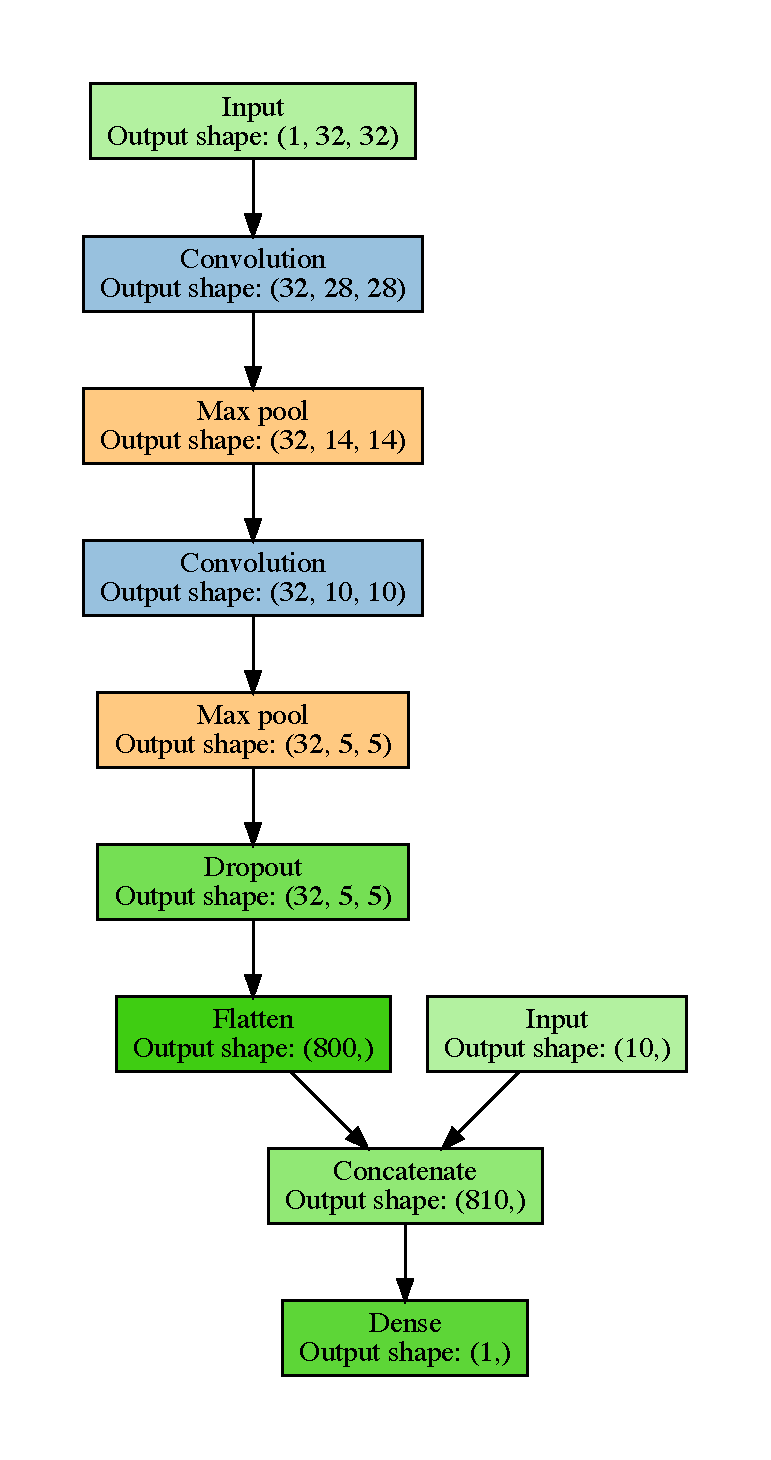
\includegraphics[width=\linewidth]{images/cnn_model_graph}
      \caption{Architecture of our CNN. The concatenate layer flattens the
      output of the previous layer and adds the 10 features derived from the
      candidate host in SWIRE, i.e. the flux ratios, stellarity indices, and
      distance. The dropout layer randomly sets $25\%$ of its inputs to zero
      during training to prevent overfitting. Diagram based on \url{
      https://github.com/dnouri/nolearn}.}
      \label{fig:cnn}
    \end{figure}

    CNNs have recently produced good results on large image-based datasets in
    astronomy \citep[e.g.][; Lukic et al. in prep]{dieleman15cnn}. We employ
    only a simple CNN model in this paper as a proof of concept that CNNs may
    be used for class probability prediction on radio images. The model
    architecture we use is shown in \autoref{fig:cnn}.

  \subsection{Random Forests}
  \label{sec:random-forests}

    Random forests are an ensemble of decision
    trees~\citep{breiman01random-forest}. They consider multiple subsamples of
    the training set, where each subsample is sampled with replacement from
    the training set. For each subsample a decision tree classifier is
    constructed by repeatedly making axis-parallel splits based on individual
    features. In a random forest the split decision is taken based on a random
    subset of features. To classify a new data point, the random forest takes
    the weighted average of all classifications produced by each decision
    tree. \edited{We used the \texttt{scikit-learn} \citep{pedregosa11sklearn}
    implementation of random forests with 10 trees, the information entropy
    split criterion and a minimum leaf size of 45}.

\section{Accuracy tables}\label{app:accuracies}
  
  This section contains tables of accuracy for our method applied to CDFS and
  ELAIS-S1. In \autoref{tab:cdfs-ba} and \autoref{tab:elais-ba} we list the
  balanced accuracies of classifiers on the cross-identification task for CDFS
  and ELAIS-S1 respectively, averaged over each quadrant. In
  \autoref{tab:cdfs-acc} and \autoref{tab:elais-acc} we list the balanced
  accuracies of classifiers on the cross-identification task for CDFS and
  ELAIS-S1 respectively, averaged over each quadrant.

  \begin{table*}
    \caption{Cross-identification accuracies for different classification
    models on CDFS. The `Labeller' column states what set of training labels
    were used to train the method, and the `Classifier' column states what
    classification model was used. `CNN' is a convolutional neural network,
    `LR' is logistic regression, `RF' is random forests, and `Labels' is the
    accuracy of the label set itself. `Perfect' indicates that the true labels
    of the test set were used and hence represents an upper bound on
    cross-identification accuracy with our method. `NN' is a
    nearest-neighbours approach. Accuracies are evaluated against the expert
    label set, so `Norris' labels are 100 per cent accurate by definition. The
    standard deviation of accuracies evaluated across the four quadrants of
    CDFS (\autoref{fig:quadrants}) is also shown.}
    \label{tab:cdfs-acc}
    \begin{tabular}{ccccc}
      \hline
      Labeller & Classifier & Mean `Compact' accuracy & Mean `Resolved' accuracy & Mean `All' accuracy\\
       &  & (per cent) & (per cent) & (per cent)\\
      \hline
      --- & NN & $97.2 \pm 1.7$ & $75.7 \pm 7.9$ & $93.4 \pm 0.8$\\
      --- & Random & $97.9 \pm 2.2$ & $22.3 \pm 9.2$ & $83.2 \pm 4.7$\\
      Norris & Labels & $100.0 \pm 0.0$ & $100.0 \pm 0.0$ & $100.0 \pm 0.0$\\
             & Perfect & $97.9 \pm 2.2$ & $99.0 \pm 1.8$ & $98.1 \pm 1.7$\\
             & LR & $97.3 \pm 0.5$ & $76.0 \pm 3.2$ & $93.7 \pm 1.8$\\
             & CNN & $96.6 \pm 0.9$ & $74.3 \pm 12.3$ & $93.5 \pm 0.5$\\
             & RF & $96.1 \pm 1.4$ & $75.8 \pm 6.7$ & $93.8 \pm 2.0$\\
      RGZ & Labels & $53.1 \pm 8.5$ & $56.7 \pm 5.9$ & $54.4 \pm 5.9$\\
          & LR & $97.3 \pm 1.9$ & $74.5 \pm 5.1$ & $93.6 \pm 1.7$\\
          & CNN & $85.4 \pm 2.6$ & $68.1 \pm 9.2$ & $92.4 \pm 1.1$\\
          & RF & $97.5 \pm 0.9$ & $74.3 \pm 7.9$ & $93.7 \pm 1.5$\\
      \hline
    \end{tabular}
  \end{table*}

  \begin{table*}
    \caption{Cross-identification accuracies for different classification
    models on ELAIS-S1. Columns and abbreviations are as in
    \autoref{tab:cdfs-acc}. Accuracies are evaluated against the expert label
    set derived from \citet{middelberg08} cross-identifications. The standard
    deviation of accuracies evaluated across models trained on the four
    quadrants of CDFS (\autoref{fig:quadrants}) is also shown.}
    \label{tab:elais-acc}
    \begin{tabular}{ccccc}
      \hline
      Labeller & Classifier & Mean `Compact' accuracy & Mean `Resolved' accuracy & Mean `All' accuracy\\
       &  & (per cent) & (per cent) & (per cent)\\
      \hline
      --- & NN & $95.5 \pm 0.0$ & $92.8 \pm 0.0$ & $95.5 \pm 0.0$\\
      --- & Random & $61.9 \pm 1.1$ & $26.6 \pm 2.1$ & $61.9 \pm 1.1$\\
      Middelberg & Perfect & $99.6 \pm 0.0$ & $99.8 \pm 0.0$ & $99.6 \pm 0.0$\\
      Norris & LR & $89.0 \pm 1.1$ & $89.7 \pm 1.8$ & $94.4 \pm 0.9$\\
             & CNN & $89.7 \pm 0.3$ & $89.4 \pm 1.4$ & $94.3 \pm 0.7$\\
             & RF & $83.8 \pm 5.6$ & $82.3 \pm 4.1$ & $90.6 \pm 2.1$\\
      RGZ & LR & $90.5 \pm 1.0$ & $92.7 \pm 0.2$ & $95.9 \pm 0.1$\\
          & CNN & $84.6 \pm 0.6$ & $84.6 \pm 0.6$ & $91.8 \pm 0.3$\\
          & RF & $91.3 \pm 1.0$ & $90.3 \pm 2.4$ & $94.7 \pm 1.2$\\
      \hline
    \end{tabular}
  \end{table*}

%%%%%%%%%%%%%%%%%%%%%%%%%%%%%%%%%%%%%%%%%%%%%%%%%%

% Don't change these lines
\bsp	% typesetting comment
\label{lastpage}
\end{document}
